%---------------------------------
% Rapport de stage de fin d'études
%---------------------------------

% Document
\documentclass[a4paper,11pt,titlepage]{report}

%---------
% Packages
%---------

\usepackage[french]{babel}
\usepackage[utf8]{inputenc}
\usepackage[table,xcdraw]{xcolor}
\usepackage[T1]{fontenc}
%\usepackage[hidelinks]{hyperref}
%\usepackage{hyperref}
\usepackage{caption}
\usepackage[top=2.3cm, bottom=2.3cm, left=3cm , right=3cm]{geometry}
% pour pieds et tete de pages
\usepackage{fancyhdr}
\pagestyle{fancy}
\usepackage{longtable}
\usepackage{enumitem}
\usepackage{lastpage}
\usepackage{graphicx}
% Use Arial equivalent on Linux
\usepackage{helvet}
\renewcommand{\familydefault}{\sfdefault}
\usepackage{float}
\usepackage{listings}
\usepackage{lscape}
\usepackage[export]{adjustbox}
\PassOptionsToPackage{hyphens}{url}
\usepackage[hidelinks]{hyperref}

\setcounter{secnumdepth}{5} %affichage numéro partie subsubsection


% Macros
\newcommand{\Author}{Raphaël GALLAIS-POU}
\newcommand{\NomDocument}{Rapport de Stage de fin d'études}
\newcommand{\VersionDocument}{1.0}
\newcommand{\RevisionDocument}{2}

\newcommand{\pathAutre}{img/other}
\newcommand{\pathPartOne}{img/part1}
\newcommand{\pathPartTwo}{img/part2}
\newcommand{\pathPartThree}{img/part3}
\newcommand{\pathPatchO}{img/appendix/patch0}
\newcommand{\pathPatchOne}{img/appendix/patch1}
\newcommand{\pathPatchTwo}{img/appendix/patch2}
\newcommand{\pathPatchThree}{img/appendix/patch3}
\newcommand{\pathPatchFour}{img/appendix/patch4}
\newcommand{\pathPatchFive}{img/appendix/patch5}
\newcommand{\pathGantt}{img/appendix}
\newcommand{\patchResults}{img/appendix/results}

% Make "Chapter N" disappear
%\makeatletter
%\def\@makechapterhead#1{%
%  \vspace*{50\p@}%
%  {\parindent \z@ \raggedright \normalfont
%    \interlinepenalty\@M
%    \Large \bfseries #1\par\nobreak
%    \vskip 40\p@
%  }}
%\def\@makeschapterhead#1{%
%  \vspace*{50\p@}%
%  {\parindent \z@ \raggedright
%    \normalfont
%    \interlinepenalty\@M
%    \Large \bfseries  #1\par\nobreak
%    \vskip 40\p@
%  }}
%\makeatother

\pagestyle{fancy}

\fancyhf{}%
\fancyhead[LO]{\bf \leftmark \medskip \smallskip}
\fancyhead[RO]{\it \medskip \smallskip \rightmark}
\fancyfoot[LO]{\sl { {\large \NomDocument \ version  \VersionDocument \ rév \RevisionDocument} }}
\fancyfoot[RO]{\thepage/\pageref{LastPage}}
\renewcommand{\footrulewidth}{0.4pt}% Line at the footer visible

\setcounter{tocdepth}{4}
\fancypagestyle{plain}{%
	\fancyhf{}%
        % Fix that
        \fancyfoot[LO]{\sl { {\large \Author} }}
	\fancyfoot[LO]{\sl { {\large \NomDocument \ version  \VersionDocument \ rév \RevisionDocument} }}
	\fancyfoot[RO]{\thepage/\pageref{LastPage}}
	\renewcommand{\headrulewidth}{0pt}
	\renewcommand{\footrulewidth}{0.4pt}
}


\title{\NomDocument}
\author{\Author}
\date{\today}

\begin{document}

%--------------
% Page de garde
%--------------

\makeatletter
	\begin{titlepage}
	\centering
		\begin{figure}[h]
			\begin{minipage}[c]{.46\linewidth}
				\centering
				
\includegraphics[width=0.8\textwidth]{\pathAutre/Logo_ESEO.jpg}
			\end{minipage}
			\hfill%
			\begin{minipage}[c]{.46\linewidth}
				\centering
				
\includegraphics[width=0.8\textwidth]{\pathAutre/Logo_STM.png}
			\end{minipage}
		\end{figure}

    \vspace{1cm}
    \vfill
%                \rule{\linewidth}{0.6mm} \\
    		{\Huge \textbf{\@title}} \\
    		\vspace{1em}
    		{\Large \textsl{CoreSight - Plateforme de Débogage}}\\
%                \rule{\linewidth}{0.6mm}
    	\vspace{10em}
    	\begin{flushleft}
		{\LARGE
                        \vspace{2em}	
        		\@author\\
        		Tuteur : Christophe ROULLIER\\
                        Référent ESEO : Mickael CLAVREUL\\
			\vspace{2em}
                        \textsl{Version : \VersionDocument\ - Révision : \RevisionDocument\\}

		}    		
    	\end{flushleft}

	\noindent\fbox {
		\parbox{\textwidth} {
		\begin{flushleft}
			{\LARGE 
				Option : Systèmes Embarqués\\
                                Entreprise d'accueil : STMicroelectronics\\
				Domaine entreprise : Automotive et IoT\\
                                Fonction du tuteur : Développeur kernel\\
				Confidentialité : niveau 0\\
			}
		\end{flushleft}
		}
    	}

    \vfill
	\end{titlepage}
\makeatother

%\include{tableVersions}

\renewcommand{\contentsname}{Sommaire}
\tableofcontents % Table des matières.
\addcontentsline{toc}{section}{Sommaire}
\listoffigures % Table des figures.
%\addcontentsline{toc}{section}{Table des figures}

%---------------------------
% Fiche de synthèse du stage
%---------------------------

\section*{Fiche de synthèse du stage}
\addcontentsline{toc}{section}{Fiche de synthèse du stage}
\label{pref:internship_synthesis}

\begin{table}[H]
\resizebox{\textwidth}{!}{%
\begin{tabular}{|c|c|}
\hline
Intitulé du stage &
  Coresight / Plateforme de Débogage \\ \hline
Date de début &
  02/03/2020 \\ \hline
Date de fin &
  28/08/2020 \\ \hline
Entreprise d'accueil &
  STMicroelectronics \\ \hline
Principales personnes impliquées &
  \begin{tabular}[c]{@{}c@{}}Christophe Roullier : Maître de stage\\ Mathieu Poirier : Mainteneur Coresight\\ Gérald Baéza et Loïc Pallardy : Architectes STM31MP1\\ Raphaël Gallais-Pou : stagiaire\end{tabular} \\ \hline
\begin{tabular}[c]{@{}c@{}}Planning résumé\\ (Réalisations personnelles)\end{tabular} &
  \begin{tabular}[c]{@{}c@{}}Prise en main de l'environnement\\ Mise en place du décodage de traces ARM Coresight\\ État de l'art du débogage interprocesseurs\\ Implémentation d'une fonctionnalité Coresight (TPIU puis ETMv3)\\ Validation de la fonctionnalité \\ Rédaction d'une documentation sur le framework\end{tabular} \\ \hline
Contraintes et difficultés rencontrées &
  \begin{tabular}[c]{@{}c@{}}État de l'art\\ Comparatif des versions des composants Coresight\\ Prise en main du framework perf\\ Implémentation de la fonctionnalité\end{tabular} \\ \hline
Résultats &
  \begin{tabular}[c]{@{}c@{}}Étude de faisabilité implémentable mais non concluante\\ Intégration de la fonctionnalité au kernel ST\\ Page Wiki disponible en interne\end{tabular} \\ \hline
\end{tabular}%
}
\end{table}
 % Fiche de synthèse du stage

%---------------------------------
% Préface - Documents obligatoires 
%---------------------------------

%--------------------
% Résumé - Abstract
%--------------------

\section*{Résumé}
\addcontentsline{toc}{section}{Résumé}
\label{pref:resume}

Ce rapport développe mon stage en ingénierie réalisé au sein de
STMicrolectronics Le Mans, dans le cadre de mon cursus d'ingénieur généraliste
à l'ESEO Angers.  On y traite de l'implémentation d'une solution de débogage
sur une carte STM32MP1 Evalboard conçue par ST. Ce stage m'a fait aborder des
sujets tels que les technologies de trace et de débogage Coresight, la
communication inter-processeurs ainsi que le développement de pilotes pour le
noyau Linux.

\section*{Abstract}
\addcontentsline{toc}{section}{Abstract}
\label{pref:abstract}

This report deals with my engineering internship carried out within
STMicrolectronics Le Mans, as part of my engineering studies at ESEO.  It
deals with the implementation of a debugging solution on a card.  STM32MP1
Evalboard. This internship made me approach subjects such as ARM Coresight
trace and debugging technologies, communication inter-processor as well as the
development of drivers for the Linux kernel.

%----------
% Mots-clés
%----------

\section*{Mots-clés}
\addcontentsline{toc}{section}{Mots-clés}
\label{pref:keywords}

ESEO, STMicroelectronics, ST, Linux, CoreSight, kernel, debug, STM32MP15x, driver, C,
OpenSTLinux, systèmes embarqués, Linux embarqué, SoC 

%--------------
% Remerciements
%--------------

\section*{Remerciements}
\addcontentsline{toc}{section}{Remerciements}
\label{pref:acknowledgements}

Je souhaite remercier mon tuteur, Christophe Roullier, pour ses conseils, son
expertise et pour m'avoir suivi et encouragé tout au long de ce projet.  Je
souhaite également remercier Mathieu Poirier, pour sa patience vis-à-vis de
mes nombreuses questions et son expertise du sous-système Coresight. Je
voudrais aussi remercier Valentin Caron pour avoir pris le temps de relire mon
rapport et pour ses remarques pertinentes ainsi que Loïc Pallardy pour son
regard critique. \\

Enfin je remercie toutes les personnes qui ont contribué à l'élaboration de
mon projet et de ce rapport ainsi que la société STMicroelectronics pour
m'avoir accueilli en tant que stagiaire. \\


%-------------
% Introduction
%-------------

\chapter*{Introduction}
\addcontentsline{toc}{chapter}{Introduction}
\label{chp:intro}

Ce stage de fin d'études de 6 mois a consisté à mettre en place une solution
permettant le débogage d'un noyau Linux embarqué dans une puce électronique
et à effectuer la validation de cette solution. \\

Ce rapport a pour but d’expliquer le déroulement de mon stage, non seulement
sur les tâches réalisées et les difficultés techniques abordées, mais
également de résumer les rapports humains auxquels j’ai été confronté. \\

Dans une première partie, je présenterai la société et le contexte de la
mission en décrivant son organisation, ses concurrents, et ses besoins grâce à
une mise en situation.  Dans un second temps je développerai quelles ont été
mes activités durant le stage en détaillant les objectifs, le cahier des
charges, les tâches réalisées, les difficultés rencontrées et leurs
résolutions.  Puis dans une dernière partie j’exposerai mon rapport personnel
lors de la mission, avec l’apport de connaissances et de savoir-faire qu’elle
a amené en insistant sur notre intégration au sein de la structure.  Enfin, je
terminerai ce rapport par une conclusion. \\


%----------------------------------------------
% PARTIE 1 : Environnement et contexte du stage
%----------------------------------------------

\chapter{Environnement et contexte du stage}
\label{chp:part1}

%--------------------
% PARTIE 1 : Contexte
%--------------------

\section{Contexte du stage}
\label{chp:part1:context}

\subsection{Présentation de l'entreprise}
\label{chp:part1:presentation_company}

STMicroelectronics (ou ST) est une société internationale d’origine
franco-italienne.  STMicroelectronics est l’un des leaders mondiaux de la
conception et fabrication de semi- conducteurs.  La société est issue de la
fusion en 1987 de deux entreprises possédées par un gouvernement
(respectivement français et italien) : Thomson Semiconducteurs et SGS
(Societa Generale Semiconduttori). Le secteur d’activité de STMicroelectronics
à cette époque a évolué de l’électronique à destination de l’énergie nucléaire
et de l’électroménager vers l’informatique et les télécommunications.  La
première entrée en bourse de ST a été en 1994 avec la bourse de Paris et de
New York.  En 1998, ST s’est positionnée comme le 14 ème fournisseur mondial de
semi-conducteurs, en 2005 comme le plus grand fournisseur européen de semi-conducteurs
, devant Infineon et NXP (ex Philips Semiconductors), et comme le 5ème
fournisseur mondial de semi-conducteurs derrière Intel, Samsung, Texas
Instruments et Toshiba. On retrouve ainsi une majorité d'entreprises
concurrentes situées aux États-Unis (Intel, Qualcomm) ainsi qu'en Asie du
Sud-Est (Samsung, Toshiba). \\

STMicroelectronics fournit un effort conséquent pour l’innovation, avec 7 400
de ses 46 000 employés travaillant en recherche et développement.
L’entreprise a déposé environ 18 000 brevets parmi 9 600 familles de brevets
différentes.  En 2018, environ 15\% des revenus ont été dédiés à la recherche
et au développement, avec 500 nouveaux brevets déposés.  Ce fort
investissement dans la recherche a permis de positionner STMicroelectronics
comme acteur clé dans les technologies nouvelles générations, avec des
microcontrôleurs très basse consommation, des composants de gestion d’énergie,
de protection, des capteurs et actionneurs MEMS, ainsi que des puces de
connectivité et de contrôle moteur. \\

Aujourd’hui, les thématiques de STMicroelectronics sont la conduite augmentée
(Smart Driving) et l’internet des objets (Internet of Things). Le secteur
internet des objets se décompose en trois sous-thématiques : les objets
connectés (Smart Things), la domotique et la ville intelligente (Smart Home
and City) et l’industrie augmentée (Smart Industry). \\

Les familles de produits issues de ces thématiques sont les circuits intégrés
numériques à applicatif spécifique (ASIC numériques), les EEPROMs et
microcontrôleurs polyvalents, les MEMS , les capteurs d’imagerie spécialisée,
les circuits intégrés analogues, industriels et de gestion d’énergie, les
circuits intégrés dédiés à l’automobile et les transistors de puissance. \\

En interne, cela se traduit en trois groupes de développement : Automobile et
circuits discrets (ADG, Automotive and Discrete IC Group), MEMS et circuits
analogiques (AMG, AnalogIC and MEMS Group) et microcontrôleurs et circuits
digitaux (MDG, Micro-controllers and Digital IC Group). \\

\begin{figure}[H]
    \begin{center}
        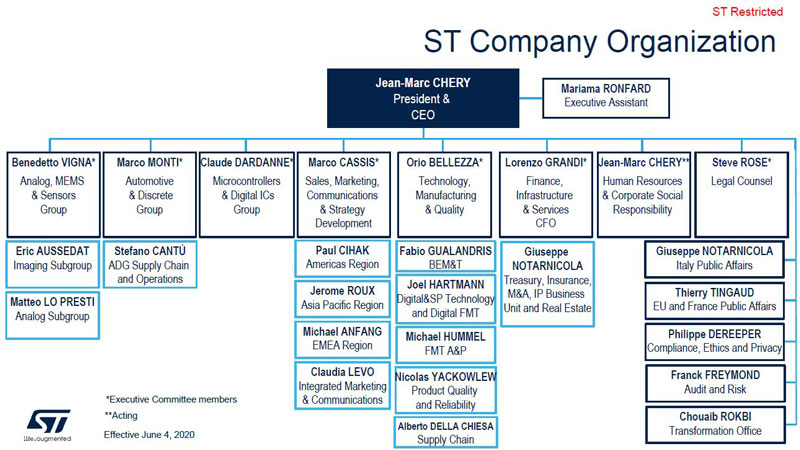
\includegraphics[width=\textwidth]{\pathPartOne/organigramme}
        \caption{Organigramme du comité exécutif ST}
        \label{fig:organigramme}
    \end{center}
\end{figure}

L’organisation hiérarchique de STMicroelectronics est très complexe du fait de
sa taille et son ampleur considérable. Dû à son affiliation franco-italienne,
l’exercice de toutes les fonctions requises pour son développement et la
gouvernance se font d’abord par un Comité de Direction. Celui-ci est composé
de huit personnes, correspondant à chaque division citée précédemment en plus
des structures financières et législatives et supervisé par M.  Jean-Marc
Chery, industriel ST diplômé de l'ENSAM Paris-Tech. Il est par ailleurs à
noter que le maintien législatif du groupe possède deux responsables des
affaires publiques pour chaque gouvernement, respectivement français et
italien. \\

À un niveau plus local, au Mans, la société Philips implémente un centre de
recherche et développement sur la technologie GSM, et fait de ce site le siège
de l’équipe « Philips Consumer Communication » en 1994. En 2001, suite à
l’arrêt pour Philips de la production de téléphones portables, une partie de
l’équipe de recherche rejoint « Philips Semiconductors » et en 2006, Philips
vend « Philips Semiconductors » qui deviendra NXP. \\

La branche «Mobile and Personal » de NXP a été cédée en 2008 au profit de la
création d’une coentreprise, ST-NXP Wireless, détenue à 80\% par
STMicroelectronics et à 20\% par NXP.  En 2009, STMicroelectronics fait
l’acquisition totale de ST-NXP Wireless pour fonder aux côtés de l’équipe «
Mobile Platform » d’Ericsson la coentreprise ST-Ericsson (détenue à parts
égales). ST- Ericsson a beaucoup contribué au développement de modems intégrés
(les NovaThor). En 2013, suite à la dissolution de ST-Ericsson, le site du
Mans rejoint STMicroelectronics. \\

\begin{figure}[H]
	\begin{center}
		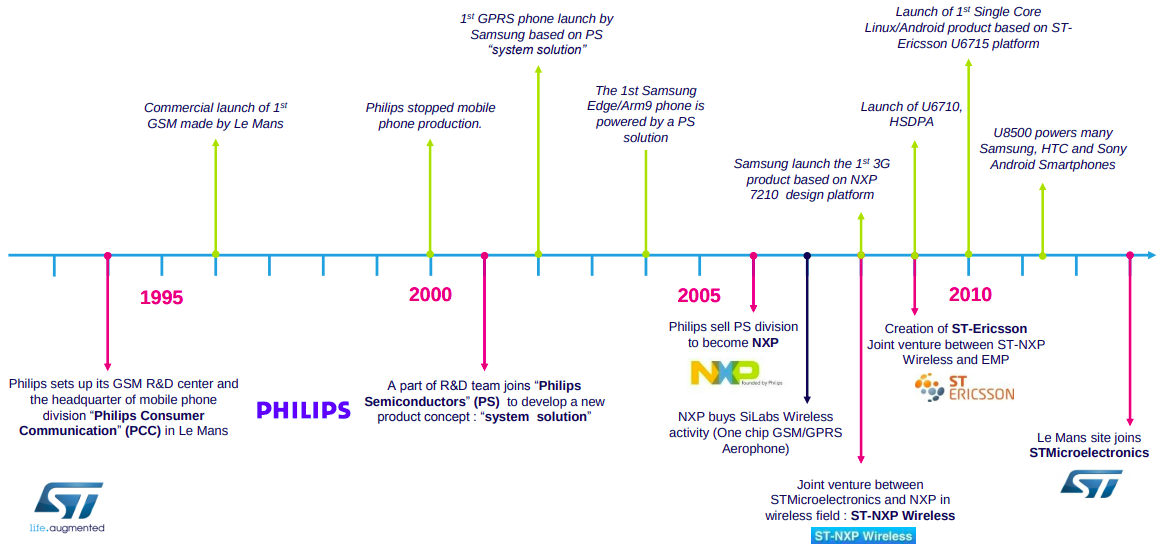
\includegraphics[width=\textwidth]{\pathPartOne/st_timeline}
                \caption{Chronogramme du site ST Le Mans}
	    \label{fig:st_timeline}
	\end{center}
\end{figure}

Aujourd'hui, le site du Mans est composé d’environ 225 employés, dont 95\%
d’ingénieurs.  Sur ces 225 employés, 118 employés (soit 52,4\%) font partie du
regroupement « Micro-controllers and Digital IC Group », 96 employés (soit
42,7\%) font partie du regroupement « Automotive and Discrete IC Group », et
enfin 11 employés (soit 4.9\%) font partie de l’équipe support. Le site du
Mans ne possède pas de division AMG. L’équipe liée au développement des
microprocesseurs (ou équipe MPU) est composée d’environ 60 employés de MDG,
dont 30 font partie de l’équipe de développement logiciel MPU dirigé par M.
Philippe Peurichard. \\

ST Le Mans est dirigé par M. Jérôme Bourgeais. Au sein de la division MPU,
parmi laquelle j'étais intégré, on retrouve des sous-groupes, nommés domaines.
Il y a par exemple le domaine Visual, traitant des pilotes autour des écrans,
touch screens et caméras, le domaine Core s'occupant de l'aspect des pilotes
Ethernet et communications ou encore Power pour la gestion de l'alimentation
du MPU. On remarquera que l'équipe "Kernel" n'existe pas pour la simple raison
que tous les domaines ont un mainteneur qui intègre le noyau Linux. \\

\subsection{Présentation des acteurs}
\label{chp:part1:presentation_actors}

Le mode de fonctionnement de cette expérience professionnelle s'inscrit dans
le cycle de développement du monde Open Source.  Effectivement, il est
désormais impossible pour une entreprise de ne pas bénéficier des logiciels
libres. En effet, chaque fonctionnalité vouée à être publiée au sein d'un
projet Open Source est passée en revue par des experts dans leur milieu. On a
donc une qualité et une sûreté de fonctionnement provenant du code intégré au
projet. Ensuite, comme l'Open Source possède l'avantage d'une gratuité de
diffusion, une entreprise lambda peut quasiment s'affranchir du coût de
maintenance puisqu'au delà de la maintenance locale à l'entreprise, des
développeurs extérieurs à l'organisation peuvent s'en charger. Enfin la
participation de nombreuses entreprises diversifie les besoins qu'un seul et
même projet doit prodiguer, et augmente par conséquent la modularité de son
code source. On retrouve ainsi une communauté d'entreprises et de particuliers
grandissante dans la participation à des projets Open Source. Pour prendre
l'exemple du noyau Linux, on retrouve de plus en plus d'applications dans le
domaine des systèmes embarqués, domaine dans lequel le noyau Linux n'était pas
destiné il y a moins d'une dizaine d'années. On peut le remarquer avec le
nombre croissant de contributeurs parmi le noyau Linux. \\

\begin{figure}[H]
	\begin{center}
		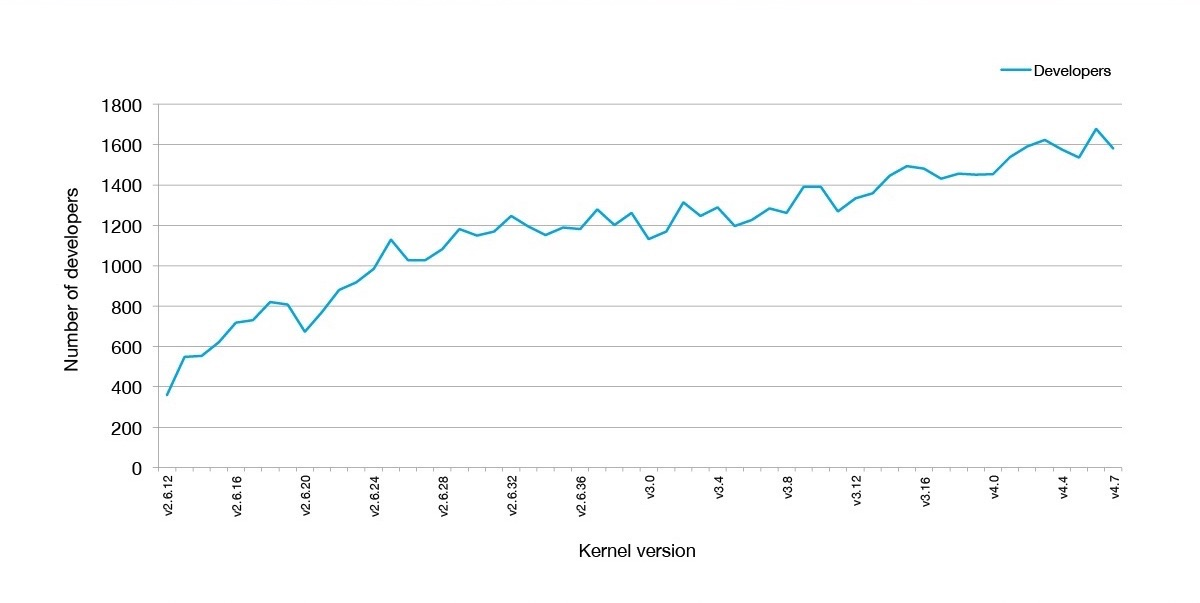
\includegraphics[width=\textwidth]{\pathPartOne/Linux-kernel-contributors-graph}
		\caption{Nombre de contributeurs au projet Linux suivant les versions}
	    \label{fig:contributors_graph}
	\end{center}
\end{figure}

Travailler au sein d'un large projet Open Source implique également un partage
à une communauté. Cette communauté se distingue en quatre catégories d'acteurs :

\begin{itemize}[label=\textbullet]
    \item Les mainteneurs
    \item Les committers ou développeurs
    \item Les contributeurs
    \item Les utilisateurs
\end{itemize}

Les utilisateurs sont les consommateurs finaux utilisant le produit. Ce sont
les acteurs les plus importants dans la mesure où ce sont eux qui répondent
directement au besoin du projet. Ici, ce sont donc les utilisateurs de la
distribution Linux publiée par ST. Les contributeurs sont des utilisateurs un
peu plus impliqués dans la conception du projet. Comme leur nom l'indique, ils
contribuent à des tâches annexes telles que la documentation, traduction,
faire des rapports de bogues sur les plateformes dédiées ou encore participent
à des campagnes de tests. Les committers sont des personnes ayant acquis une
notoriété suffisante au sein de la communauté pour s'être vu octoyer les
droits de modifier le code source. Ce sont pour ainsi dire des développeurs,
participant activement au progrès du projet. Enfin viennent les mainteneurs
qui sont des acteurs pouvant organiser des portions du code source et
approuvant l'intégration des fonctionnalités créées par les committers. Les
mainteneurs peuvent se décliner en sous-groupes de telle manière que plusieurs
mainteneurs "délégués" se chargent de l'intégration de parties spécifiques du
projet. \\

Au travers des différentes interactions entre ST et le monde extérieur, on
retrouve ainsi Linaro qui est un consortium d'entreprises dont l'objectif est
de développer et médiatiser le logiciel libre sur les architectures de type
ARM.  Linaro fait partie des 10 plus grands contributeurs au projet du noyau
Linux, et compte environ 250 ingénieurs répartis dans le monde entier. Ce
consortium inclus des entreprises telles que ARM, ST, Samsung, NXP ou encore
Google.  Parmi les acteurs décisifs de la mission qui m'a été confiée, on
retrouve Mathieu Poirier, ingénieur chez Linaro et mainteneur du sous-système
Coresight. C'est également la raison pour laquelle des échanges ont été
effectués avec lui. \\

% ARM, ST, Linaro, la communauté, Mathieu Poirier
Pour résumer, on a 4 grands acteurs de la communauté Linux pour cette mission
: ARM délivrant les blocs matériels (processeurs, sous-systèmes Coresight...),
ST chez qui le microprocesseur est conçu, et enfin Linaro. \\

\subsection{Déroulement du cycle d'un projet Open Source}

%Le cycle de développement d'un projet Open Source 
Tous ces acteurs assurent donc une pérennité du projet sur le long terme selon
un cycle de développement orienté de l'utilisateur vers le mainteneur.
L'émergeance de cette notion de remonter les informations se traduit au niveau
des committers et mainteneurs qui "upstreament" leurs nouveautés dans l'arbre
du projet principal. En pratique, les développeurs vont implémenter une
fonctionnalité répondant au besoin utilisateur et une fois validée, l'envoyer
sous forme de patch aux mainteneurs responsable de la branche. Le mainteneur
va tout d'abord inspecter si ce patch est conforme aux normes instaurées par
le projet, puis l'approuver. Dans le cas contraire, un feedback va être fait
au committer pour qu'il revoit la conception de sa fonctionnalité, d'où le
lien étroit entre développeurs et mainteneurs. Finalement, le mainteneur va
publier le patch pour une future version du projet. Cela est illustré par la
figure \ref{fig:linux_kernel_dev_process} ci-contre. \\

\begin{figure}[H]
	\begin{center}
		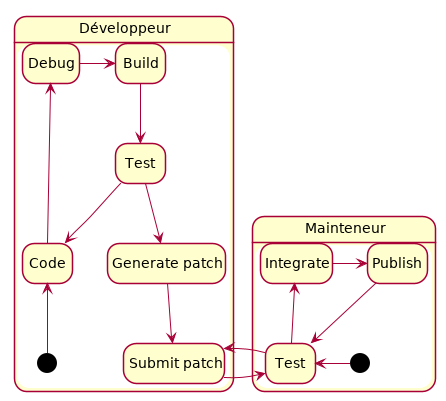
\includegraphics[scale=0.6]{\pathPartOne/linux_kernel_dev_process}
		\caption{Diagramme du processus de développement du noyau Linux}
	    \label{fig:linux_kernel_dev_process}
	\end{center}
\end{figure}

% Section économique (+ tableau?)
% Valeurs + actionnaires
% Concurrence: https://fr.wikipedia.org/wiki/Liste_des_principaux_fabricants_de_semi-conducteurs_au_fil_des_ans#Classement_2015
% Actors: https://www.linuxfoundation.org/resources/open-source-guides/participating-open-source-communities/
% Licences and juridics: https://open-source.developpez.com/tutoriels/guide-open-source/#LVII-A-2-a-i
% Linux Kernel dev process: https://www.kernel.org/doc/html/v4.15/process/2.Process.html
% https://thewalkingdeadfrance.org/global-microprocessor-market-covid-updates-3/
% https://en.wikipedia.org/wiki/Arm_Holdings

%--------------------------------------------
% PARTIE 1 : Problématique et enjeux du sujet
%--------------------------------------------

\section{Problématique et enjeux du sujet}
\label{chp:part1:issue_concern}

Grace à l'évolution de nouvelles technologies, on assiste à une
miniaturisation exponentielle des composants et une explosion de leurs
capacités. Cette croissance se retrouve dans le monde des semiconducteurs où
de nombreuses solutions se développent chaque année, répondant à divers
besoins techniques, plus particulièrement, les microprocesseurs et
microcontrôleurs. \\

Ce sont des systèmes sur puces suffisamment miniaturisés pour associer
plusieurs composants au sein d'un seul boitier. Ces Systems on Chip (SoCs)
exécutent des jeux d'instructions à la manière d'un processeur d'ordinateur.
On les retrouve dans les objets du quotidiens, tels que dans l'électroménager
ou la téléphonie mobile : des systèmes dont les capacités étaient jusqu'alors
réservées aux ordinateurs. Ces microprocesseurs présentent donc une grande
diversité dans leurs domaines d'applications. Leur présentation universelle,
mais surtout des technologies à un faible coût de revient, expliquent par
ailleurs leur production quasiment exponentielle d’année en année et leur
présence récurrente dans notre quotidien. Entre autres, on recense une
production de plusieurs millions d'unités par mois. \\

% https://thewalkingdeadfrance.org/global-microprocessor-market-covid-updates-3/
% https://www.thesneaklife.com/2020/02/06/apercu-du-marche-microprocesseur-mondial-2019-2026-intel-qualcomm-apple-amd-freescale/
% https://news.knowledia.com/CH/fr/articles/rapport-sur-le-marche-unite-de-microprocesseur-serveur-mpu-mondial-2020-37a1c04d7002644204e0163c3b8842d3e608c9c9?source=rss
% https://www.globenewswire.com/news-release/2020/02/07/1981844/0/en/Global-Microprocessors-Market-Insights-2015-2030-Green-Evolution-Has-Become-an-Urgent-Priority-for-Wireless-NSPs-and-Microprocessor-Manufacturing-Companies.html

% µProc market share: https://www.semiconductors.org/annual-semiconductor-sales-increase-21.6-percent-top-400-billion-for-first-time/
% https://www.globenewswire.com/news-release/2020/02/07/1981844/0/en/Global-Microprocessors-Market-Insights-2015-2030-Green-Evolution-Has-Become-an-Urgent-Priority-for-Wireless-NSPs-and-Microprocessor-Manufacturing-Companies.html

Le SoC STM32MP1 est la première famille de microprocesseurs commercialisée par
la société STMicroelectronics. Afin de démontrer ses capacités sur le marché,
ce microprocesseur doit faire valoir toutes ses caractéristiques. Cette
mission que l'on m'a confiée répond à un besoin interne chez
STMicroelectronics.  En effet, dans la version actuelle du microprocesseur
sont présentés des blocs hardwares non exploitables. Ces composants matériels
sont dormants en raison des pilotes (ou drivers) dont deux processeurs de la
carte ne supportaient pas jusqu'à présent.  Pourtant ces IPs sont
technologiquement les seuls moyens permettant de déboguer dans l'espace noyau.
Jusqu'à présent des solutions non conventionnelles pour investiguer des points
sur le SoC étaient présentées. Il s'agit donc d'améliorer les capacités de
débogage de l'environnement en déployant les outils communautaires et de
proposer aux clients un moyen plus ergonomique de déboguer. \\

Comme le SoC développé par STMicroeletronics possède la capacité de
fonctionner avec un OS de type Linux, il est donc soumis aux règles de la
communauté Linux. L'implémentation d'une nouvelle fonctionnalité au sein de la
carte éléctronique est également un moyen de contribution sur la communauté
Open Source. Cela permettrait donc d'enrichir le SoC et d'affirmer
STMicroelectronics comme acteur du noyau Linux. \\

À moyen et long termes, cette mission pourrait économiquement servir à gagner
des clients tant en marché de masse qu'à des entreprises consommatrices de
semiconducteurs ciblées, puisque cela servirait à déboguer plus facilement et
avec efficience. En effet, les clients vont naturellement se tourner vers des
solutions ergonomiques où il sera plus simple de développer et déboguer une
application. Ainsi s'ils ne peuvent pas le faire sur le SoC STM32MP15, ils
risquent de se tourner vers d'autres solutions, et à terme, l'entreprise
risque de perdre des clients. \\



%-------------------------------------------
% PARTIE 2 : Activités propres et détaillées
%-------------------------------------------

\chapter{Activités propres et détaillées}
\label{chp:part2}

%----------------------------------
% PARTIE 2 : Environnement technique
%----------------------------------

\section{Environnement technique}
\label{chp:part2:technical_environment}

L'intérêt de cette section est de décrire en amont les différents outils
techniques, matériels ou logiciels, qui ont dû être maîtrisés afin de mener à
bien les différentes missions qui m'ont été confiées.

\subsection{Matériel}
\label{chp:part2:subsct:hardware}

\subsubsection{STM32MP15 Wildcat}
\label{sec:wildcat_evalboard}

Le System on Chip ou SoC STM32MP15 présente sur une même puce  deux
microprocesseurs d’architecture ARM Cortex-A7 pouvant fonctionner jusqu'à une
fréquence de 800 MHz et un microcontrôleur ARM Cortex-M4 à 209 MHz. Ces trois
composants sont associés à une unité 3D GPU débouchant sur une interface
graphique MIPI-DSI et un convertisseur analogique numérique CAN.\\

Le processeur Cortex-A7 est un microprocesseur (ou MPU) performant très basse
consommation, doté d’une unité de gestion de mémoire (ou MMU), ce qui lui
permet de pouvoir exécuter un système d’exploitation. Pour le stage est
utilisé la distribution Linux open source de STMicroelectronics, OpenSTLinux,
avec le gestionnaire graphique Weston Wayland. \\

Le coprocesseur (ou MCU) Cortex-M4 est un microcontrôleur (donc dépourvu de
MMU) hautes performances et très basse consommation. Le coprocesseur est doté
d’une unité de traitement de signal (ou DSP). La présence du microcontrôleur
Cortex-M4 au sein du SoC permet de pouvoir déléguer une partie des tâches de
calculs à ce dernier, afin d’alléger la charge de travail du processeur
principal. STMicroelectronics promeut l’utilisation de l’environnement
STM32CubeMP1 pour le coprocesseur, par ailleurs, les capacités temps réel
rendent l’utilisation de RTOS ou RTEMS possible. \\

Ces deux processeurs possèdent un ensemble de périphériques qui peuvent être
soit propres à l’un des processeurs, soit partagés et donc avec la nécessité
d’être attribué à un processeur spécifique. L’attribution des périphériques
partagés s’effectue à travers le device tree, qui sera évoqué dans la partie
développement du projet. \\

\begin{figure}[H]
	\begin{center}
		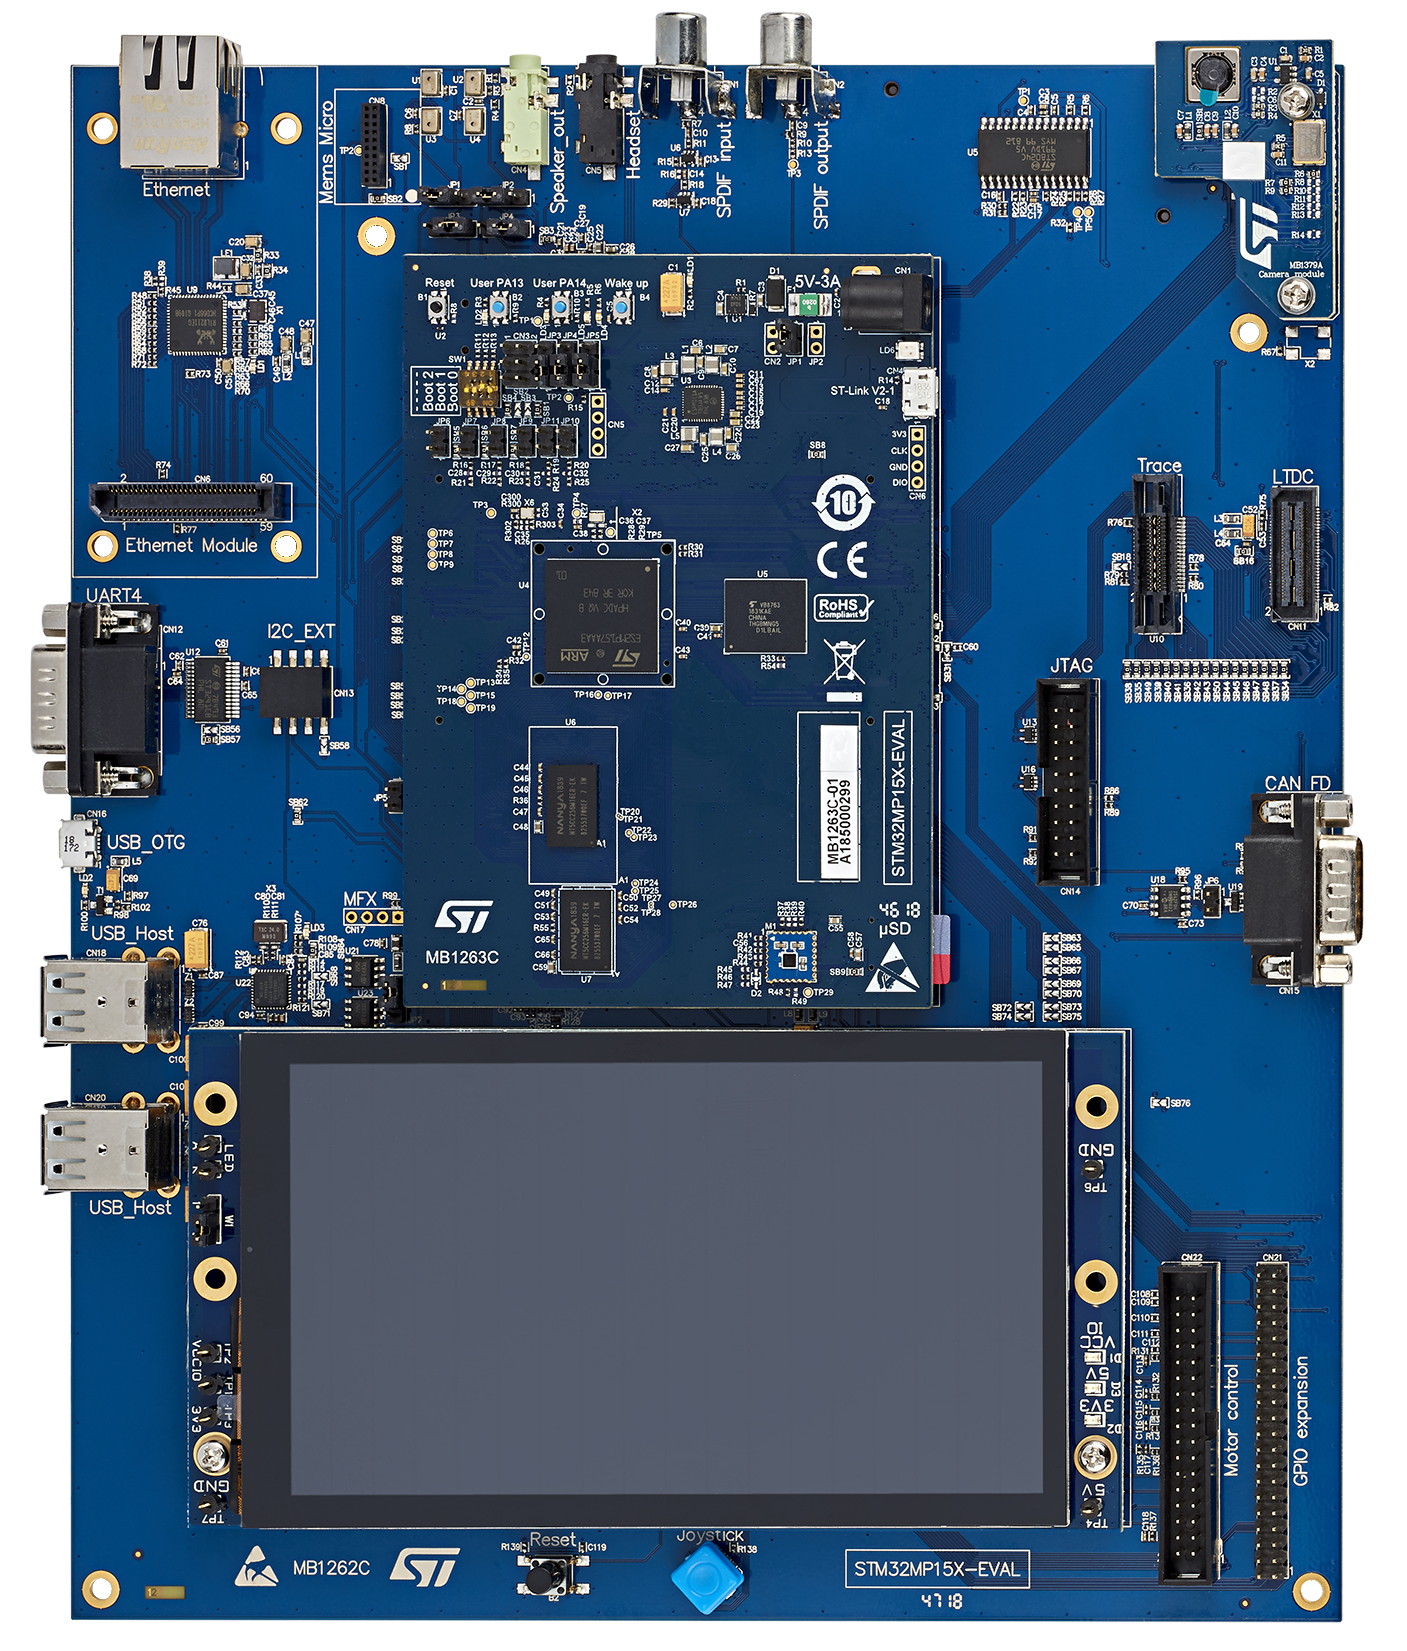
\includegraphics[scale=0.2]{\pathPartTwo/wildcat_evalboard}
		\caption{Carte référence STM32MP15 Evalboard}
	    \label{fig:wildcat_evalboard}
	\end{center}
\end{figure}

Le SoC STM32MP15 est interfacé sur la carte référence du SoC : la carte
STM32MP15 Evalboard. C'est une carte composite intégrant une carte mère sur
laquelle est soudée la puce, et une carte fille comprenant les différents
périphériques. D’un point de vue connectique, la carte comporte un connecteur
d'alimentation, un connecteur GPIO au standard Raspberry (broche de 2*20
pins), un autre utilisé spécifiquement pour le contrôle de moteur, un écran
tactile MIPI-DSI, 4 port USB-A, port micro USB On-The-Go (servant à faire
reconnaître la carte comme une clé USB), un convertisseur CAN accessible par
prise RS232, une prise RJ45 et deux prises audio jack 3.5mm. Le débogueur
embarqué ST-Link-V2 est accessible via le port UART 4 lui-même interfacé par
une prise USB-B micro. La carte contient également un port JTAG pour le
déboggage invasif. \\

Cette puce éléctronique se distingue grâce à sa connectique par ces nombreuses
fonctionnalités et augmente ainsi son champ d'application. Ses capacités et son
faible coût de revient sont également des atouts primordiaux de la puce sur le
marché.

\subsubsection{IPs CoreSight}
\label{sec:coresight_overview}

CoreSight est un nom déposé par ARM pour désigner une infrastructure de
composants électroniques permettant de tracer et déboguer des systèmes
basés sur des processeurs ARM. C'est par conséquent un nom générique pour tous
les composants ARM de traçage et débogage. \\

Les traces font référence à une quantité de données arbitraires fournissant
des informations du système à tout instant T. Ce sont ces traces, que l'on
analysera à posteriori et dont on parlera dans une section ultérieure (cf
partie \ref{sec:proper_decoding}). \\

Tout système Coresight est composé d'au moins d'un tableau de données stocké
dans une mémoire morte, appelée table ROM. Cette table en lecture seule est
accessible depuis un débogueur et fournit les adresses mémoires de tous les
composants Coresight implémentés. Dans cette table sont en réalité listés les
registres de base de chaque composant et le décalage des autres registres. En
connaissant cette adresse, en plus du décalage (ou offset) du registre que l'on
cherche à accéder, on obtient alors une cartographie de toutes les IPs ainsi
que leurs registres internes.  Le débogueur dispense ainsi d'un accès à tous
les éléments du système sans qu'il y ait un détail exhaustif de chaque
élément. \\

\begin{figure}[H]
	\begin{center}
		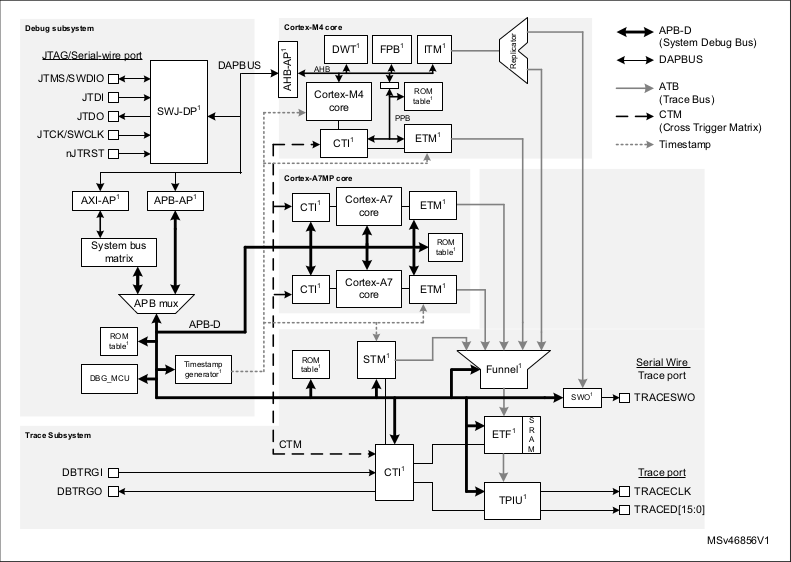
\includegraphics[width=\textwidth]{\pathPartTwo/debug_support_structure_diagram}
		\caption{Diagramme fonctionnel de l'infrastructure Coresight}
	    \label{fig:debug_support_structure_diagram}
	\end{center}
\end{figure}

Comme l'indique l'illustration \ref{fig:debug_support_structure_diagram}
ci-dessus, ce sous-système de composants s'articule autour des deux
processeurs Cortex-A7 et du coprocesseur Cortex-M4. On y observe de nombreux
composants dont certains directement impliqués dans la génération, le
transport et l'évacuation des traces Coresight. Ces derniers peuvent se
dissocier en trois catégories de composants : les sources, les puits et les
liens. \\

Les sources Coresight génèrent des données de traçage et de débogage. Ce sont
les premiers composants dans la chaîne d'acquisition de données. Dans le
système que l'on étudie, on s'attarde surtout sur les ETM (Embedded Trace
Macrocells).  Une relation de dépendance existe entre ces IPs et le processeur
sur lequel s'articule le système Coresight. Par exemple, les ETMv4 sont
spécifiques aux processeurs ARM Cortex-A8 tandis que les ETMv3 dans notre cas
s'appliquent à des Cortex-A7. De plus, selon la version de l'ETM, les capacités
diffèrent. Les ETMv1 et ETMv2, obsolètes versions des ETM, ne supportent pas
ce que les ETMv3 peuvent gérer. % Trop flou la dernière phrase 
Ces unités utilisent des bus de données de type AMBA (AHB et APB-D)
représentés sur la figure \ref{fig:debug_support_structure_diagram}. \\ 

Les liens sont des composants passifs qui peuvent s'apparenter à des
multiplexeurs et démultiplexeurs. Leur rôle est de diviser ou de multiplier
les flux de traces Coresight. Par exemple, le funnel (entonnoir en français)
est utilisé lorsqu'il y a plus d'une source génératrice. Il combine alors tous
ces flux en un seul pour aller vers un autre composant. \\

Les sinks (ou puits) permettent d'évacuer ou de stocker les traces véhiculées
au sein du système de débogage et sont les éléments finaux dans le système
Coresight. Dans le système étudié, on retrouve trois de ces IPs avec des
caractéristiques particulières. L'Embedded Trace Buffer, qui est un buffer
circulaire, fait l'acquisition des traces du système puis les stocke de
manière temporaire dans la SRAM (mémoire vive statique). Les deux autres
composants quant à eux évacuent les traces hors de la puce : le TPIU (Trace
Port Interface Unit) débouche sur le port JTAG de l'Evalboard, et le SWO
(Serial Wire Output) s'occupe d'une certaine trame, spécifique au
microcontrôleur Cortex-M4. Les deux derniers composants sont présents dans le
design hardware du système Coresight, mais restent malheureusement utilisables
en l'état. \\

Enfin, un élement central doit être mentionné puisqu'il coordonne le système.
Il s'agit du Timestamp Generator (Générateur de Timestamp). Dans un système où
plus d'un processeur est présent, il est possible que plusieurs instructions
assembleur soient exécutées quasiment en même temps par les CPUs. Dans le
résultat final il faut donc séquencer temporellement les étapes tracées. Le
timestamp generator (ou tsgen) autorise ceci en incrémentant un compteur et
envoyant à intervalles réguliers la valeur arbitraire de ce compteur. Ainsi
apparaissent dans le résultat final des trames indiquant le temps auquel les
trames se sont déroulées. Cela permet un retraçage temporel.

\subsection{Logiciel}
\label{chp:part2:subsec:software}

%\subsubsection{Environnement de développement et toolchain}
%\label{sec:env_toolchain}

%Dans une optique de praticité, les développeurs possèdent un ordinateur avec
%une distribution STUbuntu, un simple Ubuntu customisé par ST. Linux possède
%une facilité d'installation de programmes et d'outils permettant le
%développement kernel. Ainsi, une toolchain de cross-compilation est mise en
%place au lancement d'un terminal.
% what did I do in this paragraph ???

\subsubsection{GIT}
\label{sec:git}

Dans un projet d'envergure, avec une équipe de plus d'une dizaine de
personnes, il est nécessaire de hiérarchiser et d'organiser le travail et le
code source généré. Cela est possible avec GIT, un gestionnaire de version
open source et gratuit.

\subsubsection{OpenSTLinux}
\label{sec:openstlinux}

OpenSTLinux est la distribution Linux open source fournie par
STMicroelectronics pour aller sur les SoCs de type STM32MP15. C'est une
distribution basée sur Yocto, un projet facilitant la création d'outils et de
distributions Linux. Devenu un standard dans l'industrie IoT, Yocto intégre un
noyau OpenEmbedded. Le choix de ST à se tourner vers Linux, plutôt que de
créer son propre noyau fait bénéficier à l'entreprise les patchs et mises à
jour régulières faites par la communauté Linux, et permet ainsi d'avoir un
code très optimisé. 
% version avec laquelle j'ai travaillé ?

\subsubsection{Le noyau Linux}
\label{sec:linux_kernel}

\paragraph{Device tree}\mbox{}\\
\label{par:dt}

Le device tree est une arborescence de périphériques qui consiste en une
\textbf{description matérielle} de la carte électronique. Afin que le noyau
puisse effectuer des appels aux pilotes en fonction du matériel, il trouve
dans le device tree des structures de données des composants matériels tels
que les bus, périphériques, mémoires, horloges et CPU. \\

Sa finalité est donc de décrire les composants qui ne peuvent pas être
instanciés automatiquement lors du démarrage. À la différence d'une
architecture x86, ARM ne possède pas de bus avec "autodécouverte" des
composants et périphériques tel que le bus PCI. \\

Chaque fichier du device tree (.dts) est compilé individuellement par le dtc
(Device Tree Compiler) en Device Tree Blob (.dtb), mais la compilation globale
de tous les devices tree s'effectue par une règle dans le Makefile principal
du noyau : \textbf{make dtbs}. Ces devices tree blobs sont par la suite parsés et
interprétés lors de l'initilisation du noyau Linux.

\begin{figure}[H]
	\begin{center}
		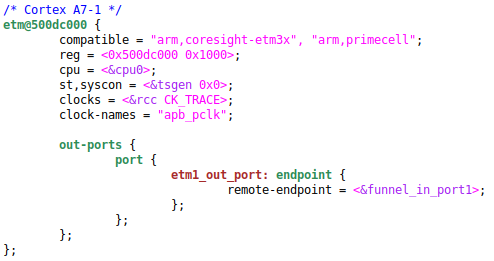
\includegraphics[scale=0.7]{\pathPartTwo/dts_etm}
		\caption{Exemple de structure du device tree d'un composant CoreSight}
	    \label{fig:dts_etm}
	\end{center}
\end{figure}

On retrouve le concept d'inclusion, à l'instar des entêtes C, donnant une
simple directive d'inclusion du contenu d'un fichier au sein d'un autre. On
retrouve ainsi des fichiers racines ".dtsi" correspondant à une description
commune entre plusieurs cartes électroniques inclus dans des device trees plus
spécifiques à chaque design. En pratique, ce fragment dtsi décrit
l'architecture interne du SoC (ici stm32MP151.dtsi). \\

Les adresses et offsets des composants sont définis dans une \textbf{memory
map} qui liste au format Excel tous les accès logiques des registres par des
bus de données. 

\paragraph{Kconfig}\mbox{}\\
\label{par:kconfig}

Au vu de la complexité du noyau Linux, de toutes les architectures existantes
ainsi que des divergences matérielles, la configuration des options du noyau
doit être simple et intuitive. Cela est rendu possible grâce à KConfig, une
interface de configuration des options du noyau. Dans chaque arborescence du
noyau, un fichier Kconfig définit les symboles et les define nécessaires à la
compilation de l'option. Pour une plus grande facilité de configuration, afin
d'éviter de passer du temps à tout configurer manuellement, une interface
utilisateur basée sur la librairie graphique NCurses est accessible avec la
commande : \textbf{make menuconfig}. Un arbre présentant toutes les options
disponibles s'affiche alors, et l'utilisateur peut choisir d'activer ou non
les options qu'il désire. En pratique, la compilation des pilotes Coresight,
primordiaux à l'utilisation du système, ne s'établie fait que si l'option est
activée à "yes".

\begin{figure}[H]
	\begin{center}
		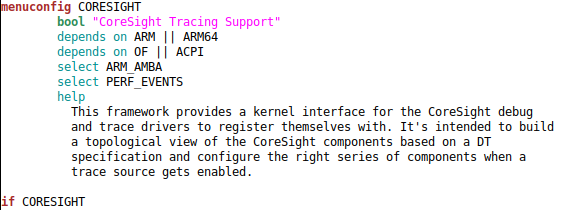
\includegraphics[scale=0.7]{\pathPartTwo/kconfig}
		\caption{Extrait de code du fichier Kconfig spécifique Coresight}
	    \label{fig:kconfig}
	\end{center}
\end{figure}

\subsubsection{Perf et le framework Coresight}
\label{sec:perf_coresight_framework}

Perf est un utilitaire Linux permettant la surveillance ainsi que le contrôle
d'évènements et la performance du noyau. Son nom est par ailleurs la
contraction du mot "performance". \\

Son code, intégré au noyau, se catégorise en deux sections : une partie espace
utilisateur qui fournit une API outil, la commande \textbf{perf} en tant que
telle, avec plusieurs sous-programmes utilitaires; et une seconde partie
espace noyau, qui gère les appels systèmes effectués dans l'espace utilisateur
et traite en conséquence les instructions reçues. \\

Cet utilitaire se base sur l'enregistrement d'évènements se déroulant à un
niveau matériel et logiciel. Cette supervision d'évènements lui confère en
conséquence la possibilité de mesurer des profils de performance avancés et de
contrôler des fonctions bas niveau. Il utilise notamment le PMU (Performance
Monitoring Unit). Ce composant, intégré dans tous les processeurs sophistiqués
produit aujourd'hui, surveille les micro évènements du CPU qu'il intègre comme
cela peut être le cas pour les cycles d'horloge écoulés, le nombre
d'instructions par cycle d'horloge ou encore le nombre de succès ou défauts de
cache. Cette PMU englobe 4 compteurs 32 bits, ainsi que des registres
spécifiques à sa configuration. \\

Chaque composant du système Coresight est instancié par des pilotes qui gèrent
séparément les IPs en elles-mêmes, mais aussi les différentes interfaces avec
leur environnement. Cela se traduit par des pilotes spécifiques pour
l'interface utilisateur sysfs ou bien des architectures pour l'intégration du
système Coresight avec l'outil perf (fichier coresight-etm-perf.c dans le
noyau). \\

Le framework et son intégration à l'outil perf rendent possible l'exploitation
dans l'espace utilisateur de profils de performance. Ces profils affichent
graphiquement ce que le processeur a exécuté. Dans le code source du noyau
Linux, les pilotes des composants sources (cf section
\ref{sec:coresight_overview}) font appel à une structure qui les modélisent en
tant que PMU. Le noyau de perf visualise ensuite cette abstraction
structurelle de la PMU lors du démarrage du noyau Linux comme le composant
utilisé. perf exerce ainsi un contrôle très précis sur l'activation et la
désactivation des traces. \\ 

\begin{figure}[H]
	\begin{center}
		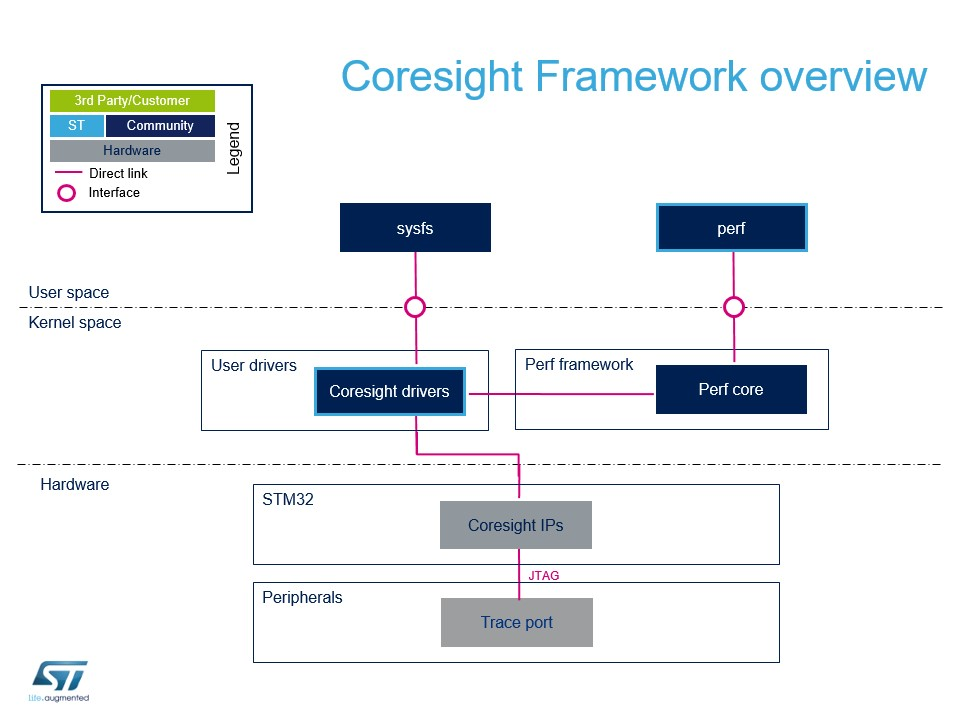
\includegraphics[width=\textwidth]{\pathPartOne/coresight_overview}
		\caption{Aperçu du framework Coresight et perf}
	    \label{fig:coresight_overview}
	\end{center}
\end{figure}
% https://01.org/linuxgraphics/gfx-docs/drm/trace/coresight/coresight.html
% search for 'coresight PMU'

%interface abstraite faisant
%l'intermédiaire entre les différents drivers PMU et le core de perf.
%cf. linaro blog from M. Poirier + Wildcat ref man
%
%
%https://unix.stackexchange.com/questions/326621/what-are-kernel-pmu-event-s-in-perf-events-list
%https://events.static.linuxfound.org/images/stories/pdf/lfcs2012_melo.pdf
%https://community.arm.com/developer/ip-products/processors/f/cortex-a-forum/5140/mrs-msr-banked-register
%https://www.kernel.org/doc/html/latest/trace/coresight/coresight.html
%https://qastack.fr/unix/326621/what-are-kernel-pmu-event-s-in-perf-events-list
%https://elinux.org/images/b/b3/Hardware_Assisted_Tracing_on_ARM.pdf
%http://rts.lab.asu.edu/web_438/project_final/Talk%209%20Performance%20Monitoring%20Unit.pdf
%https://fr.wikipedia.org/wiki/M%C3%A9moire_cache

%----------------------------------
% PARTIE 2 : Développement du stage
%----------------------------------

\section{Développement du stage}
\label{chp:part2:activities}

\subsection{Prise en main de l’environnement}
\label{sec:taking_environment}

Ma première activité a été la prise en main de l'environnement de travail et
la mise en place d'un setup fonctionnel. Il s'agit ici d'installer les outils
compilant en architecture ARM une première fois le noyau Linux ainsi que le
système opératif sur le support permettant à la STM32MP1 de démarrer, ici en
l'occurence une carte SD.

\subsubsection{Explication de la bootchain}
\label{sec:bootchain_overview}

Avant de booter Linux, un certain nombre d'étapes s'enchevêtre pour passer
d'un état inerte du système à un état où l'utilisateur le prend en main. Cette
séquence transitoire est appelée la bootchain. Lorsque l'utilisateur appuie
sur le bouton de démarrage, un microcode (ou firmware) stocké dans la mémoire
ROM (Read Only Memory), appelé le ROM code, est exécuté par le processeur afin
d'initialiser les horloges primaires. Ce ROM code appele ensuite le premier
étage de boot (FSBL) suivant le mode de démarrage choisi (par carte SD ou lien
en série). Cette étape est primordiale dans la chaîne de boot puisqu'elle doit
être sécurisée dans le but d'empêcher une potentielle vulnérabilité. C'est
pourquoi le ROM code est signé et lui-même authentifie le FSBL. \\

Une fois cet étage de boot chargé en mémoire RAM, celui-ci est exécuté. Lorque
ce dernier prend la main, il termine d'initialiser les horloges et les
premiers composants internes nécessaires au fonctionnement matériel de la
carte. Sur la STM32MP15, le FSBL implémenté est TF-A pour Trusted Firmware -
ARM. TF-A est livré par ARM à destination des processeurs Cortex A7 et A8.
Puis, ce firmware charge et authentifie le second étage de boot SSBL dans la
RAM. \\

Le SSBL instancie les fonctionnalités plus complexes et les périphériques USB,
Ethernet. Il s'occupe également de charger l'image du noyau linux dans la
mémoire vive par l'un des systèmes qu'il instancie (USB, carte SD,
Ethernet...). On pourrait faire une analogie au logiciel GRUB2 qui charge le
noyau Linux sur les architectures x86\_64. \\

Enfin l'image du noyau Linux est exécutée. Les périphériques et mémoires
externes sont reconnues, leurs pilotes instanciés, et les services Unix sont
démarrés. L'utilisateur peut finalement prendre en main la cible. \\

On se rend compte que chaque étape est un processus complexe, sujet à un
développemement ciblé en particulier, TF-A et UBoot étant des projets Open
Source à part entière. Ainsi toutes les versions entre TF-A, UBoot et le noyau
Linux ne sont pas compatibles entre elles. Un problème s'est posé lors du
rajout d'une image du noyau en version de développement 5.4 à un UBoot et un
TF-A à la version délivrée au public antérieure. Il a fallu par conséquent
compiler et écraser manuellement ces deux étages de boot par leurs versions
compatibles. 

\subsubsection{Compilation d'une image du noyau}
\label{sec:kernel_cumpilation}

Le développement du noyau Linux passe obligatoirement par une compilation du
noyau. Celle dernière est faite en plusieurs étapes, épurant le noyau dans un
premier temps, puis configurant l'image et seulement à ce moment, la
compilation et la compression peuvent avoir lieu. La première étape n'est pas
systématiquement nécessaire dans la mesure où les mainteneurs du noyau chez
STmicroelectronics s'assurent constamment d'une rétrocompatibilité.
C'est-à-dire qu'un individu lambda peut compiler un noyau Vanilla (version
sans rajouts ou modifications du noyau) et qui restera fonctionnel sur la
STM32MP15. Cette étape consiste au rajout ou retrait des fragments de
configuration caractéristiques à la carte électronique, qui imposent des
valeurs autres que celles par défaut. En réalité, il s'agit plus d'une étape
de commodité pour les développeurs au sein de l'entreprise pour éviter de
compiler des pilotes des autres architectures et ainsi gagner du temps. \\

\begin{figure}[H]
	\begin{center}
		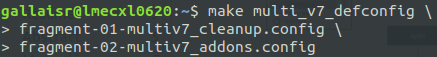
\includegraphics[scale=0.7]{\pathPartTwo/make_multiv7_dark}
		\caption{Commande utilisée pour créer la configuration}
	    \label{fig:make_multiv7}
	\end{center}
\end{figure}

Ensuite, dans le cadre du développement et de tests du noyau, la configuration
avec Kconfig (cf \ref{par:kconfig}) doit s'effectuer afin d'activer les
différents pilotes en cours de développement, comme expliqué ultérieurement.
C'est seulement, après cette étape que la compilation du noyau sera effectuée.
\\

La compilation est effectuée par le Makefile principal, situé dans la racine
du projet. Il fait appel récursivement à tous les Makefiles présents dans
l'arbre du code source. La compilation commence par synthétiser les device
trees, puis une image est formée à partir des pilotes et librairies présentes.
Cet exécutable statique \textbf{vmlinux} n'a pas de format supporté par UBoot
(cf section \ref{sec:bootchain_overview}). Une compression en spécifiant les
adresses des différents secteurs (où l'image doit être copiée dans la RAM,
l'endroit où est situé le binaire dans la partition) est faite comme le montre
l'exemple dans la figure \ref{fig:mkimage} ci-dessous. \\ 

\begin{figure}[H]
	\begin{center}
		
\includegraphics[scale=0.7]{\pathPartTwo/mkimage_dark}
		\caption{Commande utilisée pour créer l'image exploitée par UBoot}
	    \label{fig:mkimage}
	\end{center}
\end{figure}

Cette image finale doit être copiée sur la cible pour que les modifications
faites sur le noyau Linux soient prises en compte. Cela peut être réalisé par
scp si la cible est fonctionnelle et reliée au réseau ou un passage par la
console série UART avec minicom. Cette dernière méthode présente l'avantage
d'évacuer les logs de démarrage et d'exécution sur le terminal de
l'ordinateur. On peut ainsi contrôler les étapes de démarrage et les stopper
au besoin pour prendre la main sur la console des étages de boot. \\

Lorsque toutes ces étapes ont bien été executées, le démarrage de Linux a lieu
et l'utilisateur prend la main sur le système.

\subsection{Intégration de Coresight dans le device tree}
\label{sec:coresight_integration}

Pour instancier les pilotes liés aux composants Coresight pendant le démarrage
du noyau Linux, il faut dans un premier temps les assigner et les implémenter
dans le device tree.  Comme cela est expliqué dans la partie
\ref{sec:coresight_overview}, ces IPs sont internes au SoC, leur
implémentation se fait donc dans un fichier commun qui servira d'inclusion.
La description de ces IPs se fait suivant la \textbf{memory map}. Cela permet
de savoir quels sont les composants accessibles entre eux, où et comment y
accéder. \\

Chaque composant possède ainsi son propre noeud et chaque noeud va ensuite se
décliner en sous-noeuds à la manière du langage de description JSON dont une
analogie pourra être faite. Le noeud spécifie les ports entrées et sorties
présents sur le composant ainsi que des propriétés nécessaires à son
fonctionnement. Elles peuvent faire référence à une horloge, définir une
interruption ou bien être créées sur mesure. Certaines de ces propriétés sont
obligatoires pour permettre au noyau Linux de les reconnaître et de les
inclure. Typiquement, une propriété phare est la propriété \textbf{compatible}
qui associe le noeud dans le device tree à un pilote via une ou plusieurs
chaînes de caractères. Cela se traduit en pratique par une structure de
données dans le pilote appelée par le noyau lors du démarrage. Cette structure
possède un attribut \textbf{name} qui correspond à la chaîne de caractères du
compatible. Par la suite, le pilote appelle une API parser qui décomposera le
noeud en variables et appelera les fonctions en conséquences. \\

Pour prendre l'exemple de l'ETM, illustré en figure \ref{fig:dts_etm}, la
propriété \textbf{compatible} possède deux chaînes de caractères : la première
permet au pilote de reconnaître ce noeud comme étant l'ETMv3 de l'adresse
0x500DC000 ; la deuxième permet d'identifier le composant comme configurable
et non comme un composant passif. \\

Comme la nomenclature a évolué ces trois dernières années, il a fallu corriger
et améliorer le travail effectué en amont. Un avantage de l'Open Source est
que les différentes entreprises upstreament leurs device trees dans le noyau
Linux. On peut implémenter par conséquent le système présent en faisant des
analogies aux autres device trees par méthodologie comparative. \\

Implémenter le sous-système Coresight dans le device tree ne règle pas le
problème de son activation. Comme cela est expliqué dans la section
\ref{par:dt}, les noeuds Coresight du device tree ne sont appelés que par les
pilotes Coresight.  S'ils ne sont pas eux-mêmes compilés et intégrés dans
l'image du noyau Linux, leur appel n'aura pas lieu lors du boot, et les IPs
Coresight resteront dormants. Dans la configuration du noyau, les développeurs
ont créé le système de configuration Kconfig (cf section \ref{par:kconfig}).
Dans les options de configuration apparaît la macro CORESIGHT qui active
l'utilisation du système.  Des sous-options sont alors déclinées, permettant
affinant la configuration.  On peut par la suite choisir d'activer les pilotes
pour chaque composant. \\

\subsection{Décodage des premières trames Coresight}
\label{sec:coresight_traces}

\subsubsection{Choix du décodeur}
\label{sec:decoder_choice}

Pour comprendre la suite de cette section, une parenthèse est nécessaire pour
expliquer le fonctionnement des traces Coresight véhiculées au niveau
matériel. Ce flux de données, nommé \textbf{Program Flow Trace}, est généré
par les composants sources, et arrive dans un buffer ou bien est évacué par un
port JTAG. Le Program Flow Trace construit des trames à partir de différentes
instructions que le processeur effectue. En connaissance de ces étapes, en
plus de l'image du noyau Linux, on reproduit ce que le processeur a accompli,
et ainsi retrace le code exécuté à posteriori.  Seulement comme lors d'un
enregistrement, il peut se passer une infinité d'évènements (en admettant que
l'on fasse appel à un programme contenant une boucle infinie), une compression
est donc nécessaire afin de ne pas saturer le buffer de sortie. Il faudra
envisager de décoder ces traces binaires. \\

Une alternative fut prise concernant le décodage de ces traces. En effet, il
existe de nombreuses solutions, différentes les unes par rapport aux autres,
et chacune apportant ses avantages. On recense ainsi les solutions suivantes : 

\begin{itemize}[label=\textbullet]
    \item Trace32/Lauterbach
    \item DS-5
    \item ptm2human
    \item OpenCSD
\end{itemize}

L'utilisation d'un \textbf{Lauterbach}, sonde de débogage, se révèle très
pratique pour l'observation invasive du système. Cet instrument s'accompagne
d'un logiciel, \textbf{Trace32}, qui évacue des traces et les analyse
directement par le port JTAG. Cependant, c'est une technologie très coûteuse et
non accessible aux personnes de la communauté Linux. C'est pour cela qu'il n'y
a que 2 Lauterbachs sur le site de ST Le Mans et de surcroît, cette solution
n'est pas adaptée pour ce projet. De même, \textbf{DS-5} est un logiciel
propriétaire ARM de développement supportant de décodage de trace Coresight.
Une édition communautaire existe, mais elle n'implémente pas nativement ce
décodage. Il y reste donc comparativement deux dernières solutions. Ce
sont des libraires Open Source que l'on peut retrouver sur GitHub. Lorsque
l'on s'attarde sur leur code source, on se rend compte qu'\textbf{OpenCSD} est
toujours active tandis que \textbf{ptm2human} n'est plus maintenue en
apparence. Cette dernière librairie a ainsi potentiellement une obsolescence
que l'on ne retrouve pas chez OpenCSD.  Par ailleurs, OpenCSD s'intègre à
perf et permet une compilation sur cible.  C'est naturellement vers cette
solution que le projet s'est orienté pour décoder les traces Coresight.

\subsubsection{Mise en place du décodage}
\label{sec:proper_decoding}

La librairie choisie est compilée au format ARM 32 bits et x86\_64 pour
décoder des traces sur cible et sur ordinateur hôte. Une fois la librairie
enregistrée dans la toolchain aux formats ELF 32 et 64 bits, l'intégration à
l'outil perf pour chaque architecture est effectuée. Cela se fait par le
passage d'une option dans les arguments du Makefile comme le montre la figure
\ref{cmd:perf_compilation}. Cela retourne un exécutable ELF dynamiquement lié
au format 32 bits. Il ne reste plus qu'à copier les librairies et l'exécutable
sur la cible, si la commande ci-dessous a été exécutée dans l'environnement de
développement ARM. 


\begin{figure}[H]
	\begin{center}
		
\includegraphics[scale=0.7]{\pathPartTwo/make_perf_dark}
		\caption{Commande utilisée pour compiler perf}
            \label{cmd:perf_compilation}
	\end{center}
\end{figure}

\subsubsection{Enregistrement et décodage des traces}

L'enregistrement et le décodage de traces se font par deux commandes :

\begin{itemize}[label=\textbullet]
	\item \textbf{perf record}
	\item \textbf{perf report}
\end{itemize}

La première commande génère un binaire \textbf{perf.data} contenant toutes les
traces et les évènements reçus par le framework durant la commande exécutée.
Elle stocke également les librairies et modules utilisés par le noyau lors de
son exécution dans un dossier, généralement \textbf{\$HOME/.debug/}. La
seconde interprète le fichier et le dossier qu'elle affiche dans une interface
utilisateur. \\

L'intérêt de \textbf{perf record} réside dans l'enregistrement des traces
suivants plusieurs critères bien définis qui modifient l'origine de la trace,
les secteurs à enregistrer ou encore le format de la trace. 

\begin{figure}[H]
	\begin{center}
		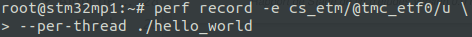
\includegraphics[scale=0.7]{\pathPartTwo/perf_record_dark}
		\caption{Commande utilisée pour enregistrer des traces}
            \label{cmd:perf_record_cs_etm}
	\end{center}
\end{figure}

Dans l'exemple ci-dessus, on cherche à mettre en évidence les différents
appels fait par la fonction \textbf{printf} aux librairies C au sein du
programme \textbf{hello\_world}. L'option \textbf{-e} désigne l'évènement qui
doit être surveillé et enregistré. Néanmoins, cette option est requise pour
utiliser le framework Coresight. Elle sélectionne en réalité l'évènement que
la PMU doit gérer.  Intrinsèquement, cela appelle l'abstraction de la PMU
faite par le framework Coresight (cf \ref{sec:perf_coresight_framework}).
\textbf{cs\_etm} identifie le composant générateur de trames Coresight et
\textbf{@tmc\_etf0} spécifie le point d'arrivée des trames. L'utilisateur peut
préférer de limiter l'enregistrement des évènements dans l'espace utilisateur
ou l'espace noyau grâce aux options \textbf{u} ou \textbf{k}. Par défaut,
lorsque cette option n'est pas spécifiée, les évènements survenant dans les
deux domaines sont capturés.  Enfin, il y a la possibilité d'effectuer des
traces suivants les threads du programme surveillé avec \textbf{--per-thread}
ou contrôler l'ensemble des CPUs avec \textbf{--all-cpus}. \\

Pour reprendre l'exemple, on enregistre ainsi les appels de fonctions de
l'espace utilisateur du programme \textbf{hello\_world} en triant ces appels
en fonction des différents threads. \\

Une fois les traces enregistrées dans le fichier \textbf{perf.data},
\textbf{perf report} affiche le profil de performance. Encore une fois,
différentes options s'offrent à l'uilisateur pour le choix de l'interface. Une
présentation des données brutes peut être faite avec :

\begin{figure}[H]
	\begin{center}
		
\includegraphics[scale=0.7]{\pathPartTwo/perf_report_dump_dark}
		\caption{Commande utilisée pour observer des traces brutes}
            \label{cmd:perf_report_dump}
	\end{center}
\end{figure}

Malgré des informations peu lisibles, cette fonction a l'avantage de présenter
directement les trames Coresight mémorisées. \\

\begin{figure}[H]
	\begin{center}
		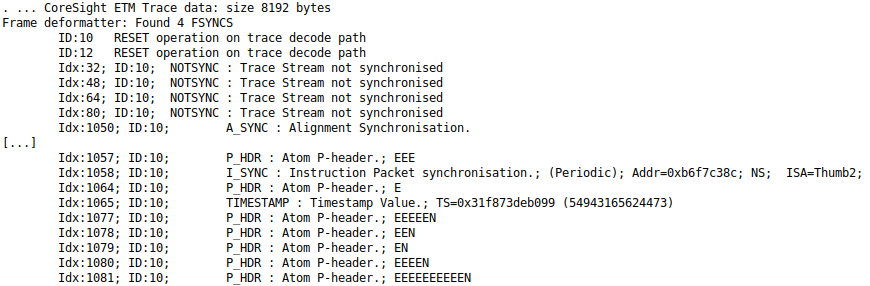
\includegraphics[width=\textwidth]{\pathPartTwo/perf_data_dump}
		\caption{Extrait du fichier perf.data à la section perf}
	    \label{fig:perf_data_dump}
	\end{center}
\end{figure}

Parmi les 8 kilooctets de données collectées, plusieurs trames sont
remarquables :

\begin{itemize}[label=\textbullet]
    \item A\_SYNC : Ce packet permet au décodeur d'aligner les trames avec leur
        adresse. Il permet au décodeur d'identifier les différents packets.
    \item Atomes P\_HDR : Ces paquets composés d'atomes, indiquent l'exécution
        des instructions. Un atome peut prendre la valeur :
        \begin{itemize}
            \item \textbf{E} indiquant que l'instruction est passée.
            \item \textbf{N} indiquant que l'instruction n'est pas passée.
            \item \textbf{W} est une valeur particulière, qui n'est pas
                applicable ici.
        \end{itemize}
    \item BRANCH\_ADDRESS (non visible sur la figure \ref{fig:perf_data_dump})
        : Les branchements sont des instructions venant interrompre
        l'exécution séquentielle d'un processeur. Ce paquet spécifie
        lorsqu'une opération de branchement survient ainsi que l'adresse de la
        prochaine instruction à exécuter.
    \item I\_SYNC : Ce packet synchronise les instructions, il renvoie
        l'adresse de l'instruction courante.
    \item TIMESTAMP (non visible sur la figure \ref{fig:perf_data_dump}) : Le
        Timestamp est une valeur arbitraire envoyée à intervalles réguliers.
        Il sert à identifier lorsque plusieurs flux de données sont présents,
        par exemple lors d'une trace sur plusieurs processeurs.
    \item CtxtID (non visible sur la figure \ref{fig:perf_data_dump}) : Ces
        paquets sont envoyés pour avertir du changement de contexte au sein du
        processeur. Ce paquet comporte l'identifiant du nouveau contexte.
\end{itemize}

Par ailleurs, chaque packet présente l'identifiant du processeur sur lequel il
est récupéré. \textbf{ID:10} désigne le premier processeur A7, et
\textbf{ID:12} désigne le second processeur. Sur la figure
\ref{fig:perf_data_dump}, on a donc une exécution du programme qui ne s'est
réalisée que sur un coeur du SoC. \\

De même, il existe une présentation plus orientée utilisateur avec :

\begin{figure}[H]
	\begin{center}
		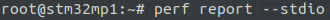
\includegraphics[scale=0.7]{\pathPartTwo/perf_report_stdio_dark}
		\caption{Commande utilisée pour observer des traces formatées}
            \label{cmd:perf_report_stdio}
	\end{center}
\end{figure}

L'option \textbf{--stdio} affiche le résultat comme un texte. Par défaut,
l'application utilise la librairie graphique NCurses. Dans une mesure de
simplification de la présentation, on utilise le format texte. \\

\begin{figure}[H]
	\begin{center}
		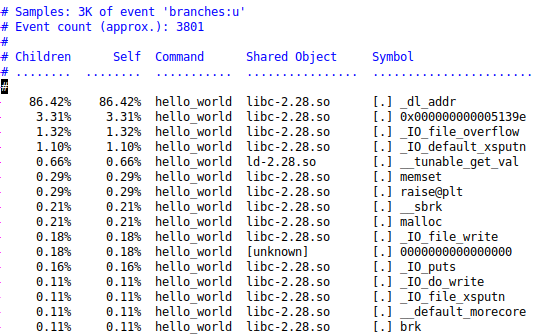
\includegraphics[width=\textwidth]{\pathPartTwo/perf_data_stdio}
		\caption{Extrait du fichier perf.data à la section perf}
	    \label{fig:perf_data_sdtio}
	\end{center}
\end{figure}

Sur l'image \ref{fig:perf_data_sdtio} ci-contre on observe donc les
différentes fonctions appelées par la commande supervisée. \\

L'aperçu du résultat montre d'abord une approximation du nombre d'évènements
reçus. Puis, sont affichées 5 colonnes chacune ayant une signification bien
précise.  Les deux premières colonnes \textbf{Children} et \textbf{Self}
désignent le pourcentage de temps passé dans la fonction appelée par rapport
au temps total d'exécution. La somme de ces pourcentages est normalement égale
à 100\% pour la colonne "Self", tandis que ce n'est pas un cas systèmatique
pour "Children". Cela est dû au calcul du temps. Children représente la somme
du temps passé dans les processus fils. La troisième colonne, explicite,
précise qu'elle était la commande supervisée lors de l'appel. Dans le cas
présent, c'est le programme \textbf{hello\_world}. La quatrième et la dernière
colonne font respectivement référence à la librairie utilisée et la fonction
appelée, appelée aussi symbole, dans cette librairie. Dans le cas où le
symbole n'est pas reconnu, perf pointe vers son adresse. Lorsque l'échantillon
mesuré provient du noyau, la référence à la librairie est remplacée par
\textbf{[kernel.kallsyms]} et le \textbf{[.]} signifiant l'espace utilisateur
du symbole est remplacé par \textbf{[k]}.

\subsection{État de l'art du débogage interprocesseurs}
\label{sec:faisabilite_m4}

Une étude annexe a consisté à faire un état de l'art concernant le débogage
interprocesseurs. \\

L'Evalboard possède 3 coeurs : 2 processeurs ARM Cortex-A7 et un coprocesseur
ARM Cortex-M4. Généralement, les coeurs des deux processeurs délèguent les
tâches de calculs au coprocesseur. Cela explique l'idée de vouloir déboguer le
troisème coeur par l'intermédiaire des coeurs A7. Cette mission a ainsi pour
objet de vérifier si l'utilisation des IPs Coresight pour récupérer les traces
du Cortex-M4 est possible. \\

Pour comprendre la stratégie de développement, une discussion avec Mathieu
Poirier, expert Linaro a été entamée. Ce dernier a expliqué que, dans le cas
où l'ETM appartenant au domaine du coprocesseur était accessible depuis l'un
des deux processeurs Cortex-A7, il suffisait seulement à le configurer pour
l'activer.  Cela serait possible puisque les traces qu'il produit atterrissent
directement dans le ETF, buffer de sortie commun avec les traces des deux
coeurs A7. \\

Aussi dans un premier temps, il a fallu comprendre si les différents registres
de l'ETMv3 du coprocesseur étaient accessibles depuis les deux coeurs ARM
Cortex-A7.
 
\subsubsection{Analyse préliminaire}
\label{sec:initial_analysis}

Les processeurs et le coprocesseurs n'appartiennent pas au même domaine dans
la mémoire. Leurs registres et périphériques associés sont séparés, et les
accès mémoires passent par l'intermédiaires de bus de données ne communiquant
pas directement. Dans le domaine des processeurs, les composants Coresight
utilisent le bus \textbf{APB-D} tandis que ceux du coprocesseur utilisent le
bus \textbf{AHB}. Des ports permettant des échanges sont accessibles à
différents bus et permettraient d'accéder aux registres des composants
Coresight du coprocesseur. Ces deux ports \textbf{AHB-AP} pour le bus AHB et
le port \textbf{APB-AP} pour le bus APB-D communiquent par un troisième, le
\textbf{DAPBUS} que la figure \ref{fig:bus_ports} met en valeur.  Dans une
mesure de sécurité, la communication entre ces différents bus n'est possible à
condition qu'un espace mémoire pour les IPs soit implémenté dans chaque bus,
et que des signaux d'authentification soient activés par le \textbf{BSEC}.  \\

\begin{figure}[H]
	\begin{center}
		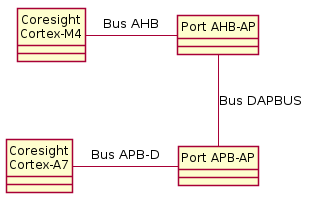
\includegraphics[scale=0.7]{\pathPartTwo/bus_ports}
		\caption{Diagramme d'accès aux bus}
	    \label{fig:bus_ports}
	\end{center}
\end{figure}

Ce périphérique interne est destiné à configurer le SoC et ses paramètres de
sécurité via le contrôle d'une puce. En particulier, il possède un registre
\textbf{BSEC\_DENABLE} définissant les signaux d'authentification nécessaires
au déboguage du SoC qui seront utilisés. Parmi les signaux utiles, on retrouve
:

\begin{itemize}[label=\textbullet]
    \item DBGEN (bit 1) qui active le débogage.
    \item NIDEN (bit 2) qui active le débogage non-invasif.
    \item DEVICEEN (bit 3) qui autorise l'accès aux composants Coresight par
        un port extérieur.
    \item DBGSWENABLE (bit 10) qui active l'accès logiciel aux composants
        Coresight.
\end{itemize}

Ce registre est accessible à l'adresse 0x5C005014 grâce à un utilitaire
similaire à busybox, \textbf{devregs} qui lit et écrit à l'adresse donnée si
le registre le permet. La lecture du registre renvoie 0x0000047F. Les signaux
listés sont donc activés et la valeur renvoyée laisse penser par conséquent
que l'implémentation d'une solution pour un dégogage interprocesseurs est
possible.

\subsubsection{Ajout de l'ETM du coprocesseur au device tree}
\label{sec:add_etm_m4_dt}

Intuitivement et aux vues de la description qu'il a fallu ajouter et modifier
dans le device tree, une première étape fut d'instancier l'ETM dans le device
tree, à l'instar des deux ETM dédiés aux processeurs Cortex-A7. L'ETM du
coprocesseur se situe à l'adresse 0xE0041000 dans la memory map. \\

L'instanciation de l'ETM est faite dans le device tree à l'adresse indiquée
ainsi que les branchements au funnel pour pousser les traces en sortie (cf
\ref{fig:debug_support_structure_diagram}). Une fois le noyau Linux démarré,
on vérifie l'état de l'ETM ; ce qui est fait par la lecture avec devregs du
premier registre des ETMs du coprocesseur, de valeur initiale 0x00000411 et
d'un processeur en tant que témoin, l'\textbf{ETMCR} qui possède un offset en
mémoire de 0x000 et une valeur par défaut de 0x00000461. Celui-ci montre la
valeur 0xbff5f77b, différente de celle par défaut (0x00000411) tandis que
l'ETM du processeur vaut bien la valeur par défaut (0x00000461). \\

Le coprocesseur étant dormant à ce niveau de l'étude, cela expliquerait le
comportement de l'ETM. Un firmware est téléversé sur le microcontrôleur afin
de le démarrer avant le noyau Linux. Cependant, malgré l'activation du
microcontrôleur, le démarrage du noyau est impossible en raison d'une erreur
persistante. Cette erreur engendre un blocage lors de l'initialisation d'un
périphérique du STM32MP15 qui ne peut alors plus démarrer.

\subsubsection{Vérification dans la memory map}
\label{sec:mmap}

En regardant sur la memory map de la puce électronique, on se rend compte que
l'adresse normalement occupée par l'ETM du coprocesseur est réservée à la
mémoire DDR, et que seul le débogueur peut accéder à cette adresse. Une
explication possible de la valeur en apparence arbitraire du registre
s'expliquerait par une lecture dans une zone réservée de la mémoire. La memory
map montre également qu'il n'y a pas d'emplacement dédié à l'ETM du
coprocesseur parmi les bus de communication des processeurs. \\

L'étude menée se révèle ainsi non concluante car les IPs Coresight du
coprocesseur ne sont pas accessibles depuis les processeurs. Un phénomène
intéressant en revanche est notable : les accès mémoires autorisent une
lecture/écriture des registres des IPs Coresight dédiés aux Cortex-A7 depuis
le coprocesseur.  \\

Dans un second temps, on souhaiterait partir de la communication existante
entre le A7 et le coprocesseur pour lancer une trace sur le M4 et recevoir les
infos de débogage par les processeurs. Le coprocesseur, non autonome pour
cette partie-là, serait alors un "esclave" des processeurs. \\

Au sein du noyau Linux, il existe un système de boîte aux lettres, appelé
remoteproc, par lequel les processeurs et le coprocesseur communiquent.  Comme
le montre la figure \ref{fig:coprocessor_management} suivante, cette
communication se base sur une mémoire partagée entre les trois coeurs du
système. Il faudrait ainsi créer un protocole de communication spécifique pour
du débogage avec Coresight et implémenter dans la HAL (Hardware Abstraction
Layer) des pilotes configurant les registres des IPs Coresight. Le
coprocesseur activerait par la suite son système selon la demande faite par
remoteproc et enverrait les évènements et les traces à l'ETF pour qu'il les
intégre. \\

\begin{figure}[H]
	\begin{center}
		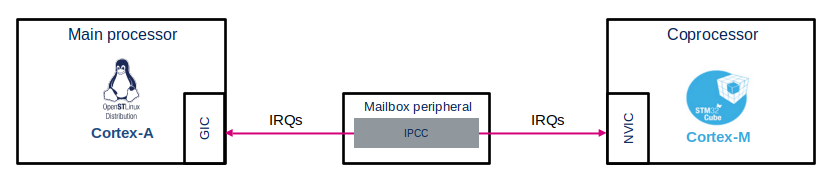
\includegraphics[width=\textwidth]{\pathPartTwo/coprocessor_management}
		\caption{Diagramme fonctionnel de l'infrastructure Remoteproc}
	    \label{fig:coprocessor_management}
	\end{center}
\end{figure}

Une solution pourrait être ainsi implémentable sur une vision au long terme.
Un tel développement, en prenant en compte la conception du protocole de
communication, l'implémentation des pilotes Coresight du coprocesseur dans le
cas où ils n'existent pas, prendrait entre deux à trois ans à temps plein pour
deux ingénieurs (un ingénieur par tache). En considérant l'intégration de ce
système avec perf, il faudrait au moins deux ans supplémentaires pour arriver
à un système fonctionnel. L'idée de déboguer le coprocesseur est donc
abandonnée pour ce projet.

\subsection{Ajout de fonctionnalité à perf}
\label{sec:add_perf_feature}

En étudiant le code source des pilotes Coresight, le TPIU apparaît comme
incomplet. Celui-ci étant un \textbf{pilote bouchonné}, par conséquent qui ne
fait rien d'autre que de renvoyer un résultat prédéfini ou une erreur, il
aurait été judicieux de l'implémenter. En effet, cette IP débouche sur le port
JTAG. À moyen terme pour valider le travail effectué, il aurait fallu passer
par un décodage des traces avec \textbf{Lauterbach}. Comme cela a été évoqué
en section \ref{sec:decoder_choice}, peu de clients risquent de l'utiliser en
raison de son coût. Aussi, l'implémentation de ce pilote a été abandonnée.
Néanmoins, au cours de l'étude de faisabilité, une erreur a été detectée lors
de la collecte d'une trace. Effectivement, lors d'une trace au niveau du noyau
avec un échantillonage de tous les CPUs (directive \textbf{--all-cpus}), un
crash de perf est observé.  En regardant les appels systèmes de perf avec
l'utilitaire \textbf{strace}, on observe la lecture d'un registre d'un ETMv4
avant le crash de l'application.

\subsubsection{Problématique d'implémentation}
\label{sec:problem_implementation}

Cette référence aux registres de l'ETMv4 est due en partie au travail effectué
autour du framework Coresight et de son intégration dans perf. En effet,
l'ETMv4 n'est pas une version supportée par un processeur Cortex-A7, mais par
un Cortex-A8, plus puissant que le Cortex-A7. La demande client auprès de ce
processeur étant plus grande, les développeurs s'attardent plus sur ce
processeur et ses périphériques. De plus le Cortex ARM V8 n'est compatible
qu'avec l'ETM en version 4. \\

L'utilisation intensive du débogueur GDB sur les cas générants un crash de
perf a permit l'identification d'un problème : le traitement de l'ETMv3 est
écarté. Le code source de perf se voulant générique, la création d'un objet
\textbf{cs\_etm} autorise une interface standard entre perf et les différentes
versions des ETM dans l'espace utilisateur. C'est donc cet objet que perf
appelle lors de l'échantillonage des traces et qui effectue les appels
systèmes au noyau en conséquences. L'objet configure par la suite une
structure de données selon la version de l'ETM et retourne un pointeur vers
cette structure. \\

Au sein de cet objet, un test est passé pour connaître l'origine de l'ETM en
fonction de l'identifiant du CPU qui lui est donné en argument. Puis, la
configuration diffère suivant le booléen retourné. Ce test est effectué dans
la fonction \textbf{cs\_etm\_is\_etmv4}, dont on peut voir le prototype
ci-dessous.

\begin{lstlisting}[language=C]
static bool cs_etm_is_etmv4(struct auxtrace_record *itr, int cpu)
\end{lstlisting}

Dans cette fonction, l'interface sysfs est utilisée pour scanner les fichiers
des registres en lecture seule. Suivant la présence ou non d'un fichier
correspondant à un registre spécifique de l'ETMv4, une valeur est renvoyée.
C'est ensuite en fonction de ce booléen qu'une erreur est renvoyée par le
programme. Considéré comme étant critique dans la configuration de perf, rien
n'est enregistré et la commande s'arrête. Cette fonction est notamment appelée
dans les fonctions responsables de la configuration du \textbf{ContextID} et
du \textbf{Timestamp}. \\

Cette gestion de l'ETMv3 non implémentée explique ainsi le comportement de
perf lors de l'échantillonage de tous les CPUs. 

\subsubsection{Comparaison entre les registres de l'ETMv3 et l'ETMv4}
\label{sec:etmv3_etmv4_comparison}

Pour comprendre la logique d'implémentation, et notamment quelles sont les
fonctions des registres de l'ETMv4 qui ont été gérées, une étude comparative
entre les registres de l'ETMv4 et l'ETMv3 utilisés a été menée. Ces registres
apparaissent dans le sysfs en lecture seule à titre informatif de l'état et
des capacités de l'ETM. La lecture dans l'interface sysfs est obligatoire
puisque la partie espace utilisateur du code de perf ne peut pas accéder
directement aux registres.

\paragraph{Timestamp}\mbox{}\\
\label{par:timestamp}

\begin{lstlisting}[language=C]
static int cs_etm_set_timestamp(struct auxtrace_record *itr,
				struct evsel *evsel, int cpu)
\end{lstlisting}

Dans la fonction de gestion du timestamp ci-dessus, le registre
\textbf{TRCIDR0} de l'ETMv4 est lu par l'interface sysfs, puis stocké dans une
variable. Ce registre de 32 bits en lecture seule indique les capacités de
traçage de l'ETMv4. Il possède notamment un mot \textbf{TSSIZE} de 5 bits
consacré à la taille du timestamp. Ce mot peut prendre 3 valeurs :

\begin{itemize}[label=\textbullet]
    \item 0 (0b00000 en binaire) dans le cas où le timestamp n'est pas
        supporté
    \item 6 (0b00110) pour signifier que le timestamp sera encodé sur 48 bits.
    \item 8 (0b01000) pour signifier que le timestamp sera encodé sur 64 bits. 
\end{itemize}

\begin{figure}[H]
	\begin{center}
		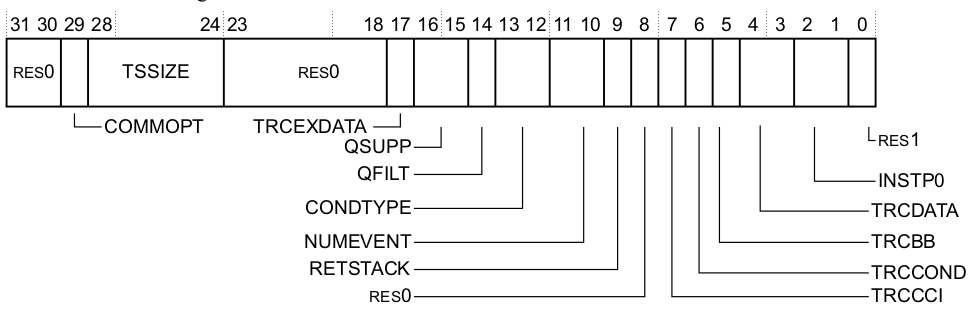
\includegraphics[width=\textwidth]{\pathPartTwo/etmv4_trcidr0_register}
		\caption{Aperçu du registre TRCIDR0 de l'ETMv4}
	    \label{fig:etmv4_trcidr0_register}
	\end{center}
\end{figure}

Par la suite dans la fonction de configuration du timestamp, un
\textbf{masque} de la taille du mot \textbf{TSSIZE} est appliqué sur la
variable contenant la valeur du registre afin de l'isoler. Elle est testée
dans une condition pour connaître si l'ETM supporte le traçage du timestamp.
Enfin elle avertie le noyau Linux de la configuration. Dans le cas contraire
la fonction renvoie une erreur. \\

Dans la documentation du SoC, un registre de l'ETMv3 est en rapport avec le
Timestamp : \textbf{ETMCCER} (ETM Configuration Code Extension Register).  Il
possède le même champ \textbf{TSSIZE} que le registre de l'ETMv4 et le champ
\textbf{TIMSTMP}. À la différence de l'ETMv4, ces mots sont encodés sur 1 bit.
De plus, c'est TIMSTMP qui définit si le timestamp est supporté, TSSIZE ne
fait qu'indiquer la taille du tmestamp. Ainsi si TIMSTMP vaut 0, la
fonctionnalité de timestamp n'est pas implémentée.

\begin{figure}[H]
	\begin{center}
		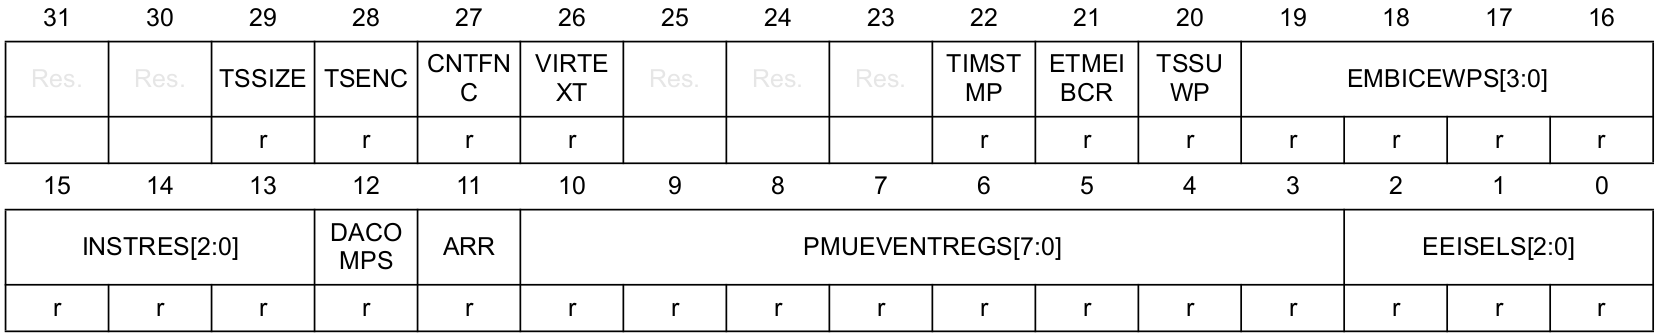
\includegraphics[width=\textwidth]{\pathPartTwo/etmv3_etmccer_register_2}
		\caption{Aperçu du registre ETMCCER de l'ETMv3}
	    \label{fig:etmv3_etmccer_register}
	\end{center}
\end{figure}

Comme ce registre apparaît en lecture seule, il est immuable. Une vérification
de sa valeur en passant par sysfs montre que le bit 22 correspondant à
\textbf{TIMSTMP} est à 1. L'ajout du registre est donc possible. Pour ce
faire, le retour d'erreur précédemment cité en section
\ref{sec:problem_implementation} est remplacé par la lecture de ce registre,
puis une condition est ajoutée pour effectuer le traitement de la valeur du
registre et l'avertissement de la configuration au noyau Linux. Ce
séquencement est illustré par la figure \ref{fig:cs_etm_set_context_id},
commun avec la section suivante.

\paragraph{Context ID}\mbox{}\\
\label{par:contextid}

\begin{lstlisting}[language=C]
static int cs_etm_set_context_id(struct auxtrace_record *itr,
				 struct evsel *evsel, int cpu)
\end{lstlisting}

La fonction de la configuration du Context ID se comporte d'une manière
similaire à la fonction liée au timestamp. Le registre utilisé a plusieurs
taches, dont celle d'indiquer la taille de l'adresse de l'instruction exécutée
et celle d'indiquer la taille du Context ID. Cette dernière tache est
appréhendée par un mot \textbf{CIDSIZE} de 5 bits sur le deuxième octet du
registre (figure \ref{fig:etmv4_trcidr2_register}). Lorsque la valeur de ce
mot vaut 0 (0b00000 en binaire), le ContextID n'est pas supporté par l'ETMv4 ;
donc il ne créera pas ce paquet dans le flux de traces. Dans le cas où il vaut
4 (0b00100 en binaire), cela signifie que le Context ID est supporté et que sa
taille peut atteindre 32 bits au maximum. Les autres valeurs de cet octet sont
ignorées. L'information utile de ce registre est de montrer que le Context ID
est supporté sur l'ETM. 

\begin{figure}[H]
	\begin{center}
		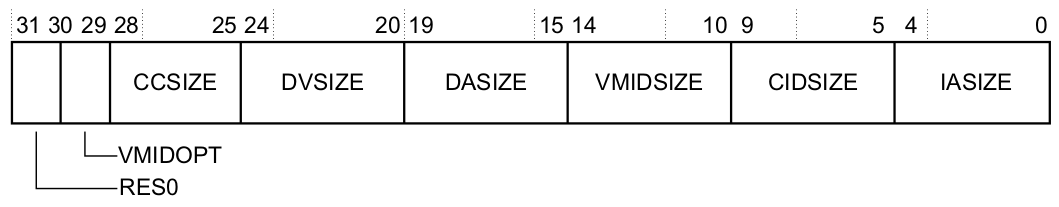
\includegraphics[width=\textwidth]{\pathPartTwo/etmv4_trcidr2_register}
		\caption{Aperçu du registre TRCIDR2 de l'ETMv4}
	    \label{fig:etmv4_trcidr2_register}
	\end{center}
\end{figure}

Deux registres dans l'ETMv3 y réfèrent et potentiellement pourraient être
l'analogue du registre TRCIDR2 dans l'ETMv4. \\

Le premier, dont on reviendra en section \ref{sec:clocks_and_tsgen}, est le
registre de contrôle général de l'ETM : \textbf{ETMCR} (ETM Control Register).
Ce registre en lecture/écriture possède un champ de 2 bits dédié à la taille
du Context ID. Il peut prendre les valeurs suivantes :

\begin{itemize}[label=\textbullet]
	\item 0 ou 0b00
	\item 1 ou 0b01 
	\item 2 ou 0b10 
	\item 3 ou 0b11 
\end{itemize}

Dans le cas où ce champ vaut 0, le Context ID n'est pas supporté. Dans les
autres cas, cela indique quelles sont les tailles du Context ID. \\

Le second registre est un registre de configuration en lecture seule :
\textbf{ETMCCR} (ETM Configuration Code Register). La documentation précise
qu'il "permet au logiciel de lire la configuration [...] de l'ETM, donnant le
nombre de chaque type de ressource". À l'instar de l'ETMCR, il possède un mot
\textbf{CONTXTIDCMP} de 2 bits, et indique le nombre de comparateurs utilisés
(pouvant aller jusqu'à 3) pour créer le Context ID. Si sa valeur est à 0, il
n'y a pas de comparateurs et le Context ID n'est pas supporté. Dans le
STM32MP15, il n'y a qu'un comparateur, la valeur du CONTXTCMP affichée par
défaut dans sysfs est 1 (0b01).

\begin{figure}[H]
	\begin{center}
		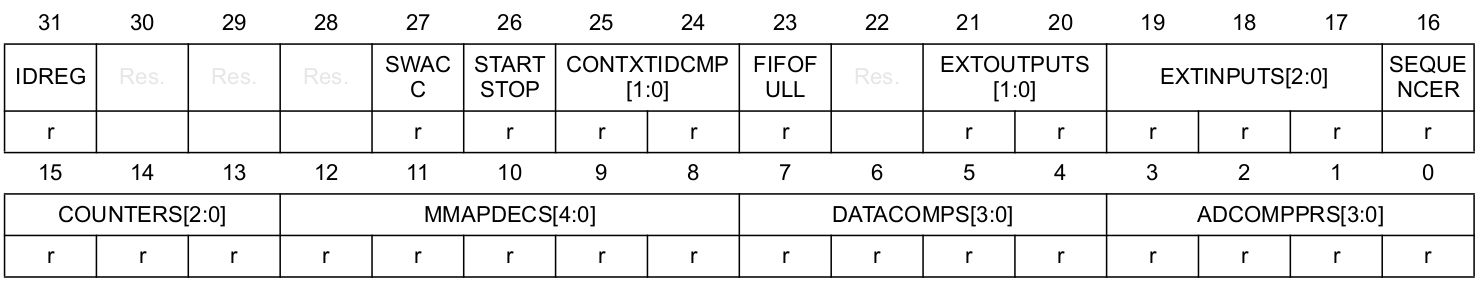
\includegraphics[width=\textwidth]{\pathPartTwo/etmv3_etmccr_register_2}
		\caption{Aperçu du registre ETMCCR de l'ETMv3}
	    \label{fig:etmv3_etmccr_register}
	\end{center}
\end{figure}

L'\textbf{ETMCR} est d'abord implémenté de la même manière que le registre de
l'ETMv4 \textbf{TRCIDR2} en prenant compte de la gestion d'erreur. Un échange
avec Mathieu Poirier pour discuter de l'implémentation révèle que le mot
CONTXTIDSIZE de l'ETMCR est un masque de bit à tracer et non à lire.
C'est-à-dire que l'écriture dans ce registre affecte la configuration
générale de l'ETM, comme son nom l'indique. L'implémentation avec ce registre
ainsi abandonnée, puis remplacée avec l'\textbf{ETMCCR}. Au final, les deux
fonctions modifiées ressemblent à la figure \ref{fig:cs_etm_set_context_id}
ci-dessous. \\

Une campagne de tests montre que les traces enregistrées proviennent bien des
deux processeurs Cortex-A7. Cela est fait par l'exécution d'un programme en
espace utilisateur contenant deux threads. Pour s'assurer que ces deux threads
s'exécutent bien sur les deux coeurs et non en alternance sur un seul coeur,
leur affinité est associée pour chaque coeur, dans un premier temps. Ensuite,
après avoir vérifié que l'affinité de Linux exploite bien tous les coeurs
présents par défaut, un simple programme exécutant deux threads est utilisé
dont le code source se trouve en annexe. \\

\underline{\textbf{Note : }} Sur le diagramme ci-dessous est représenté en
bleu les étapes déjà implémentées et en beige les étapes qui ont été ajoutées. 

% trace.affinity.all-cpus.2020_06_05_150756.tgz

\begin{figure}[H]
	\begin{center}
		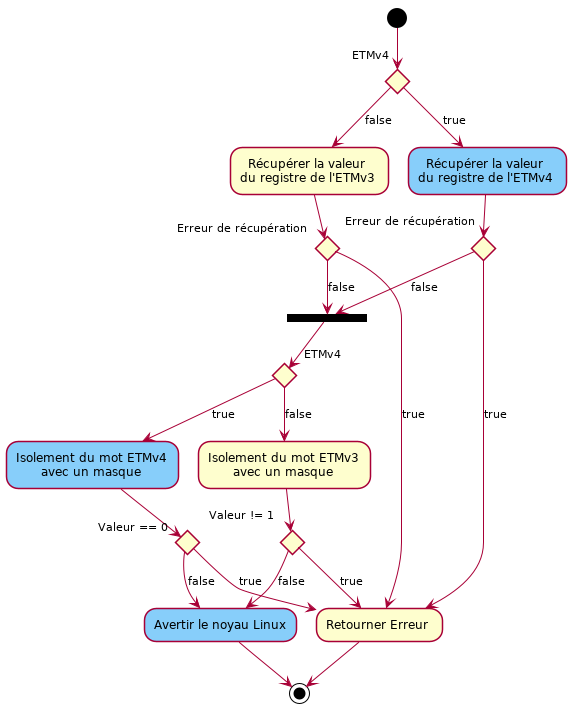
\includegraphics[scale=2.5]{\pathPartTwo/cs_etm_set_context_id}
		\caption{Algorithme des fonctions de configuration du timestamp et du Context ID}
	    \label{fig:cs_etm_set_context_id}
	\end{center}
\end{figure}

\subsubsection{Gestion des horloges et du générateur de timestamp}
\label{sec:clocks_and_tsgen}

Après avoir vérifié que les trames proviennent des deux coeurs Cortex-A7, une
première étape de validation a été menée avec une revue du résultat par
Mathieu Poirier. Cependant, d'après lui, un paquet essentiel, celui du
\textbf{TIMESTAMP}, est absent dans les traces. Il horodate les paquets et
permet ainsi de les organiser chronologiquement. \\

Une méthode naïve serait de forcer les bits des registres activant les
fonctionnalités nécessaires telles que les horloges et le générateur de
timestamp. En effet, le registre \textbf{ETMCR} contient un attribut
\textbf{TSEN} de 1 bit. Celui-ci permet d'activer l'horodatage. De plus, ce
registre n'est modulable que dans le pilote de l'ETMv3 puisque il est en
lecture/écriture. Le code du pilote est modifié en forçant ce bit, puis une
image est recompilée. La commande \textbf{perf record} est exécutée sur le
programme \textbf{thread} mentionné précédemment. L'analyse du perf.data
révèle la présence de trames de timestamp dans le fichier, mais le compteur du
générateur de timestamp ne s'incrémente pas. Les paquets de timestamp envoyés
restent ainsi à 0 comme le montre l'extrait ci-dessous. Cela explique
l'absence de trames de timestamp observée précédemment dans les traces. \\

\begin{figure}[H]
	\begin{center}
		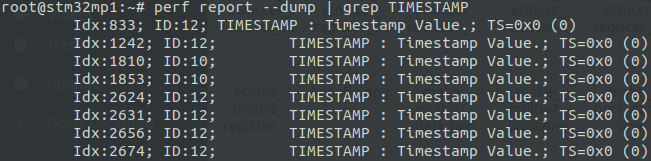
\includegraphics[width=\textwidth]{\pathPartTwo/perf_report_timestamp_0_dark}
		\caption{Extrait des trames TIMESTAMP nulles du fichier perf.data}
	    \label{fig:perf_report_timestamp_0}
	\end{center}
\end{figure}

\underline{\textbf{Note : }} On peut observer sur l'extrait ci-dessus que les
trames TIMESTAMP sont générées sur les deux processeurs, avec leur identifiant
\textbf{ID:10} et \textbf{ID:12}. \\

Cette étape n'étant qu'une étape de diagnostic du problème, une implémentation
plus élaborée et "upstreamable" doit être conçue, car tous les SoCs utilisant
ce pilote ne font pas face à ce problème. On sait que le registe
\textbf{ETMCCER} mentionné en \ref{par:timestamp} est défini lors de
l'implémentation, et possède un bit identifiant si le timestamp est supporté
par l'ETMv3. Ainsi, il faut encapsuler ce "diagnostic" dans une condition
permettant de vérifier si le timestamp est supporté. En pratique, une
structure \textbf{drvdata} est véhiculée au sein du pilote. Cette structure
contient les spécificités associées à une instance de l'ETM, telles que son
adresse d'accès ou le CPU et les horloges auxquelles il est attribué. Cette
structure spécifie également les valeurs des registres ETMCCR et ETMCCER. On
peut donc récupérer la valeur du mot \textbf{TIMSTMP} en l'isolant grâce à une
opération bit à bit. Puis, si cette valeur vaut 1, signifiant que le timestamp
est implémenté, alors on l'active dans l'ETMCR. La figure
\ref{fig:driver_etmv3_code_1} ci-dessous illustre cette implémentation.

\begin{figure}[H]
	\begin{center}
		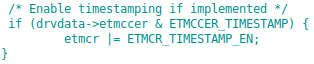
\includegraphics[scale=0.8]{\pathPartTwo/driver_etmv3_code_1}
		\caption{Extrait du code du pilote gérant l'ETMv3}
	    \label{fig:driver_etmv3_code_1}
	\end{center}
\end{figure}

Les traces Coresight présentant des paquets TIMESTAMP nuls, il faut maintenant
trouver comment avoir des valeurs incrémentées.  Après avoir consulté les
archives de mails Coresight et la documentation de l'IP, on s'aperçoit que le
registre de contrôle du compteur \textbf{TSG\_CNTCR} possède un bit EN
consacré à l'activation de l'incrémenteur du tsgen (figure
\ref{fig:tsg_cntcr_register}). Celui-ci est en en lecture/écriture et la
memory map annonce son adresse à 0x50082000.  Après vérification manuelle du
registre en utilisant \textbf{devregs} le bit EN apparaît à 0, montrant ainsi
que le compteur de l'incrémenteur est désactivé. \\

\begin{figure}[H]
	\begin{center}
		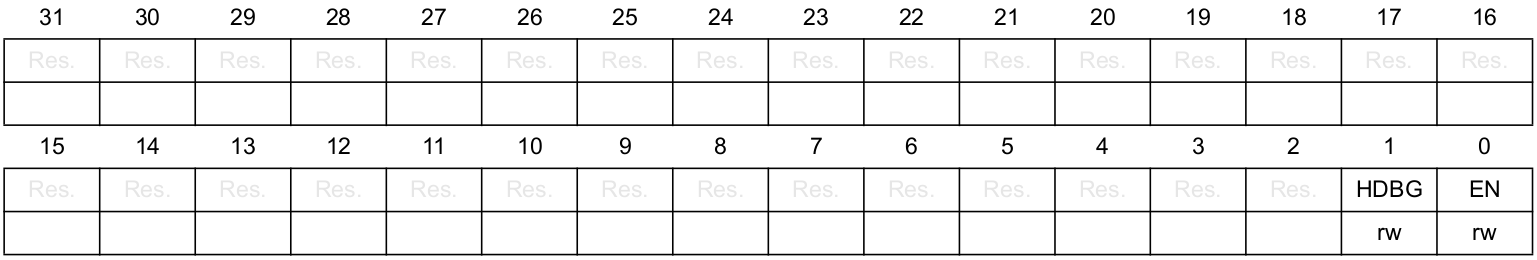
\includegraphics[width=\textwidth]{\pathPartTwo/tsg_cntcr_register_2}
		\caption{Aperçu du registre TSG\_CNTCR du Timestamp Generator}
	    \label{fig:tsg_cntcr_register}
	\end{center}
\end{figure}

Pour activer ce bit à 1, plusieurs méthodes sont possibles :

\begin{itemize}[label=\textbullet]
	\item Stopper l'exécution avant le démarrage du noyau Linux
		manuellement et passer par la console pour l'activer .
	\item Activer ce bit avec l'utilitaire devregs, toujours manuellement,
		avant l'exécution de perf record.
	\item Activer ce bit par défaut dans la configuration du système.
	\item Trouver une solution pour le faire dynamiquement.
\end{itemize}

L'idéal est d'automatiser cette activation afin que le client ait le moins
d'étapes à effectuer pour obtenir son résultat. Les deux premiers points sont
donc utilisés uniquement à des fins de validation du problème. Aussi le bit
est activé avec \textbf{devregs} avant le lancement d'une trace. Le perf.data
résultant montre que la valeur des paquets de timestamp s'incrémentent bien.
La modification du registre \textbf{TSG\_CNTCR} est donc responsable de
l'apparition de timestamps valides. \\

\begin{figure}[H]
	\begin{center}
		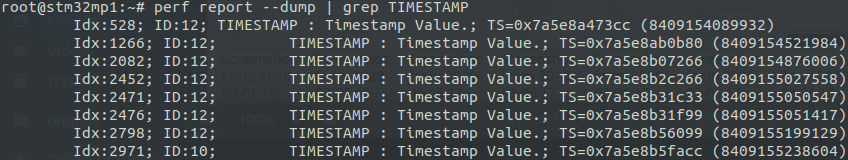
\includegraphics[width=\textwidth]{\pathPartTwo/perf_report_timestamp_dark}
		\caption{Extrait des trames TIMESTAMP du fichier perf.data}
	    \label{fig:perf_report_timestamp}
	\end{center}
\end{figure}

Ensuite, après discussion avec l'architecte du projet STM32MP15 et Mathieu
Poirier, l'activation par défaut de cette horloge n'était pas envisageable
dans un soucis de consommation superflue de la carte életronique et d'une
activation systématique malgré une utilisation ponctuelle. Il a fallu donc
trouver une solution pour activer dynamiquement cette horloge, lorsque l'IP
Coresight de l'ETMv3 est présente au sein du SoC. \\

De même, deux méthodes se présentent :

\begin{itemize}[label=\textbullet]
	\item Implémentation d'un pilote pour le tsgen.
	\item L'utilisation d'un noeud dans le device tree. \\
\end{itemize}

L'implémentation d'un pilote dédié à la gestion du générateur de timestamp est
séduisante dans la mesure où elle se base sur la détection automatique du
composant en le cherchant à travers le bus AMBA. Cela est possible puisque
tout système Coresight ne possède qu'un timestamp generator. Comme
l'activation ne concerne qu'un bit dans la configuration des registres du
tsgen, on pourrait tout aussi bien passer par un noeud arbitraire implémenté
dans le device tree. Ainsi cela permettrait aux constructeurs n'ayant pas
cette horloge par défaut de pouvoir l'activer sans crainte de gêner ceux
l'ayant par défaut. \\

\begin{figure}[H]
	\begin{center}
		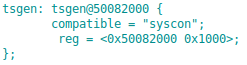
\includegraphics[scale=0.8]{\pathPartTwo/tsg_dt_property}
		\caption{Extrait du device tree, avec la propriété ajoutée}
	    \label{fig:tsg_dt_property}
	\end{center}
\end{figure}

Par mesure de simplicité, la deuxième méthode d'implémentation a été choisie.
Un noeud décrivant le timestamp generator a donc été rajouté dans le device
tree, que la figure \ref{fig:tsg_dt_property} met en valeur. En addition, une
propriété est ajoutée dans les noeuds des ETMs pour faire référence à
l'utilisation de cet IP. Cette propriété est possible grâce au pilote
MFD/syscon. C'est un framework implémenté dans le noyau dont la vocation est
d'uniformiser l'implémentation de pilotes par une API. Le pilote syscon en
particulier (SYStem CONtroller) permet ainsi un accès à divers registres de
configuration n'ayant aucun lien matériel entre eux. \\

La gestion du noeud et de la propriété dans le device tree se traite lors de
l'appel de la fonction \textbf{etm\_probe()} pendant l'initialisation du noyau
Linux. Il faut modifier cette fonction pour que la propriété soit lue, et
analyser en conséquence suivant les cas où elle ne serait pas présente dans
une autre configuration du device tree. Un booléen \textbf{tsgen\_active} est
ainsi initialisé suivant la présence ou non de cette propriété. Dans le cas où
elle est absente, aucune opération n'est réalisée. Dans le cas échéant, la
propriété pointant vers le noeud du tsgen, est alors lue et l'adresse du tsgen
est stockée dans une structure \textbf{regmap} (REGister MAP). Si la lecture
de la propriété échoue, une erreur est renvoyée comme la figure
\ref{fig:Activation_TSGEN} le met en valeur. Cette structure regmap interface
le registre \textbf{TSG\_CNTCR}, et permet au pilote de le modifier.  Ainsi
avec l'API regmap, le bit est modifié conformément à l'activation du compteur.

\begin{figure}[H]
	\begin{center}
		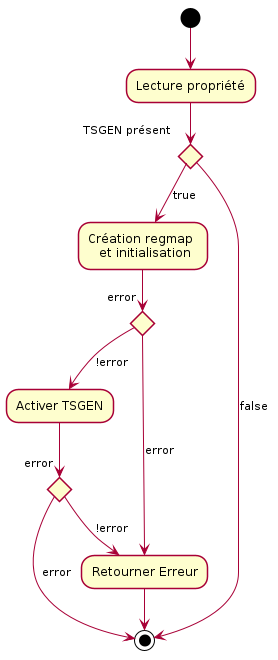
\includegraphics[scale=0.5]{\pathPartTwo/Activation_TSGEN}
		\caption{Diagramme de l'algorithme d'activation du tsgen}
	    \label{fig:Activation_TSGEN}
	\end{center}
\end{figure}

\subsection{Validation fonctionnelle et documentation}
\label{sec:validation_tests}

\subsection{Revue par les pairs}
\label{sec:peer_review}

Une fois l'implémentation effectuée, (cf figure \ref{fig:Activation_TSGEN}),
une première validation officieuse de l'implémentation par les pairs est
faite. Le code produit est soumis à Mathieu Poirier sous forme de patchs, qui
permet au développeur et mainteneurs d'échanger d'importantes quantités de
code sans les inconvénients d'envoyer tous les fichiers modifiés. \\

Après examen, Mathieu révèle qu'une solution meilleure est de créer
directement un pilote \textbf{coresight-tsg} dédié à la gestion du générateur
de timestamp. Comme c'est également le mainteneur du sous-système Coresight au
sein du noyau Linux, le code ne peut pas être upstreamé, car son aval n'est
pas approuvé compte tenu de la solution retenue.

\subsubsection{Scénarios de tests}
\label{sec:tests}

Pour valider cette fonctionnalité, des scénarios de tests sont mis en place.
Ils couvrent notamment les cas d'utilisation suivants :

\begin{itemize}[label=\textbullet]
	\item Les traces sont lancées à un espace utilisateur.
	\item Les traces sont lancées à un espace noyau.
	\item On peut enregistrer les traces sur l'ensemble des threads. 
	\item On peut enregistrer les traces sur l'ensemble des deux
		processeurs.
	\item On peut enregistrer des traces avec d'autres options de
		formatage.
	\item On peut analyser les traces brutes enregistrées.
	\item On peut analyser les traces formatées enregistrées.
\end{itemize}

Des tests nominaux sont ensuite effectués :

\begin{enumerate}
	\item perf record -e cs\_etm/@tmc\_etf0/u --per-thread ./thread
	\item perf record -e cs\_etm/@tmc\_etf0/k --all-cpus ./thread
	\item perf record -e cs\_etm/@tmc\_etf0/k --per-thread ./thread
	\item perf record -e cs\_etm/@tmc\_etf0/u --all-cpus ./thread 
\end{enumerate}

Dans les deux derniers scénarios nominaux, un affichage des données de manière
formatée ne s'effectue pas, cependant ces cas affichent bien les données
brutes. De plus, dans chaque cas les Context ID et Timestamps des traces
montrent qu'elles proviennent bien des deux processeurs. D'autres tests
couvrants plus de cas sont ensuite effectués avec différents programmes pour
s'assurer qu'ils passent bien avec divers types de programmes. Ils prennent
aussi en compte divers options de formatage en sortie et des évènements à
tracer en particulier. Un exemple de trace analysées se trouve en annexe. Les
résultats sont disponibles ci-dessous :

\begin{table}[H]
\centering
\begin{tabular}{|c|c|}
\hline
Scénario de test                                                                                             & Analyse des données \\ \hline
Scénario nominal 1                                                                                           & Brutes + formatées  \\ \hline
Scénario nominal 2                                                                                           & Brutes + formatées  \\ \hline
Scénario nominal 3                                                                                           & Brutes              \\ \hline
Scénario nominal 4                                                                                           & Brutes              \\ \hline
Traces noyau par CPU avec timestamp                                                                          & Brutes + formatées  \\ \hline
\begin{tabular}[c]{@{}c@{}}Traces noyau par CPU avec contextID\\ et formatage par instructions\end{tabular}  & Brutes + formatées  \\ \hline
\begin{tabular}[c]{@{}c@{}}Trace noyau par CPU avec timestamp \\ et formatage par branchements\end{tabular}  & Brutes + formatées  \\ \hline
\begin{tabular}[c]{@{}c@{}}Trace noyau par CPU avec timestamp \\ et avec instructions par cycle\end{tabular} & Brutes              \\ \hline
\begin{tabular}[c]{@{}c@{}}Trace utilisateur par thread \\ avec programme "uname"\end{tabular}               & Brutes + formatées  \\ \hline
\begin{tabular}[c]{@{}c@{}}Trace utilisateur par thread\\  avec programme "thread"\end{tabular}              & Brutes + formatées  \\ \hline
\end{tabular}
\end{table}

\subsubsection{Rédaction de la documentation}
\label{sec:wiki}

Enfin, une documentation doit être mise en place pour expliquer au client le
fonctionnement de Coresight, ce qu'il peut lui apporter et comment prendre en
main le framework. Un Wiki public est ainsi en cours d'élaboration au moment
où ce rapport est rédigé. Il décrit d'un côté le système d'un point de vue
matériel, le rôle des composants principaux et apporte plus de précision sur
le framework et son intégration avec perf d'un autre côté. \\

Le but de ces articles est également d'illustrer avec des examples pour que le
client puisse prendre en main le système le plus efficacement possible. Le
processus de validation de ces articles est effectué en deux temps. D'une part
des retours internes sont faits à l'aide de remarques à l'auteur de l'article
et ensuite, une fois que l'article est suffisamment élaboré pour le considérer
terminé, il est alors rendu disponible publiquement aux clients. De plus, dans
un soucis de communication universelle, les articles sont rédigés en anglais.

% perf script cs-trace-disassembly.py non existent
% https://lists.linaro.org/pipermail/coresight/2020-May/004009.html

%---------------------------------------
% PARTIE 2 : Organisation et déroulement
%---------------------------------------

\section{Déroulement et bilan technique}

\subsection{Planning prévisionnel}

\begin{figure}[H]
	\begin{center}
		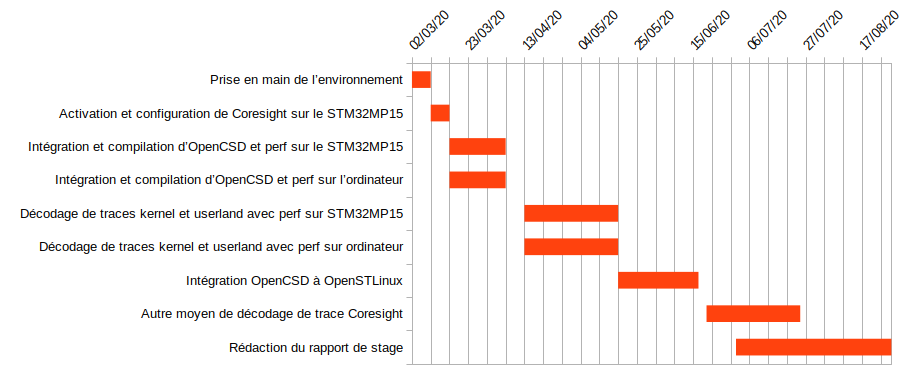
\includegraphics[width=\textwidth]{\pathPartTwo/gantt_previsionnel}
		\caption{Diagramme de Gantt du planning prévisionnel}
	    \label{fig:gantt_previsionnel}
	\end{center}
\end{figure}

\subsection{Planning effectif}

\begin{figure}[H]
	\begin{center}
		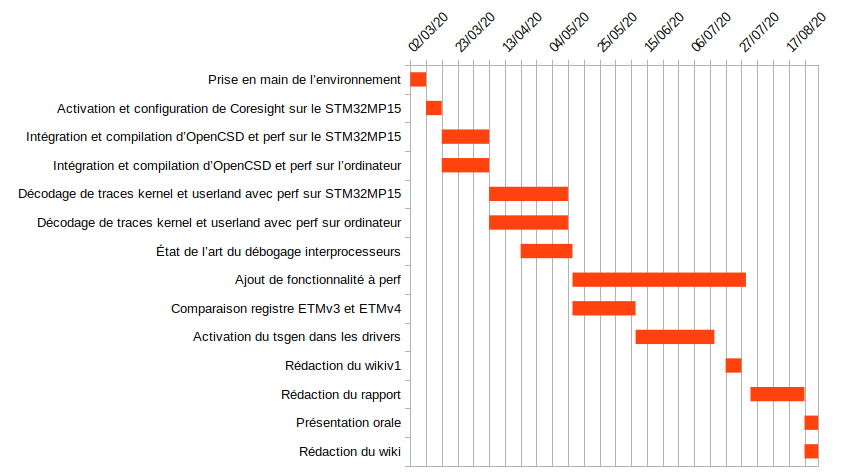
\includegraphics[width=\textwidth]{\pathPartTwo/gantt_effectif}
		\caption{Diagramme de Gantt du planning effectif}
	    \label{fig:gantt_effectif}
	\end{center}
\end{figure}

\subsection{Apport environnemental}
\label{sec:environmental_benefits}

En terme d'apport vis-à-vis de l'entreprise, plusieurs éléments auront été
légués à STMicroelectronics. Tout d'abord, même s'il n'y a pas eu de
document écrit concernant l'état de l'art du débogage interprocesseurs,
une réponse et une potentielle solution ont été données à l'oral lors de la
réunion organisée pour rendre compte de cette mission annexe. \\

De plus, le code source modifié sous forme de patchs a été envoyé sur le dépôt
GIT de l'entreprise. Une sauvegarde du code produit est disponible pour les
personnes souhaitant y accéder. Ce code, étant une solution temporaire à une
demande de l'entreprise, est par ailleurs en cours d'intégration au sein de la
branche ST du noyau Linux. Il comporte 7 fichiers et comptabilise 326 lignes
ajoutées et 27 retirées.  Le client, lors de l'utilisation de la distribution
fournie par ST, pourra ainsi utiliser le système Coresight puisqu'il sera
activé spécifiquement sur les cartes STM32MP15. Cela permettra par ailleurs de
déboguer les applications et programmes conçus au sein de l'espace noyau. \\

Enfin, la documentation des composants et du framework réalisée sur le Wiki
permet aux différents utilisateurs et aux clients une publication des
connaissances accumulées pendant le stage ainsi que la possibilité de
comprendre comment ce système fonctionne.

\subsection{Critique objective}
\label{sec:perf_criticism}

\subsubsection{perf}

Au vu du planning prévisionnel, la possibilité du développement d'un driver
Linux n'avait pas été prise en compte. Dans le planning effectif, le projet
s'est développé en cinq étapes : La prise en main et activation du
sous-système Coresight, l'intégration et le décodage de traces, l'état de
l'art du débogage interprocesseurs et enfin l'ajout de la fonctionnalité au
sein de perf. \\

Ayant eu auparavant une expérience avec la STM32MP1 lors d'un précédent
projet, la prise en main et l'activation de l'environnement ont été très
rapide.  De même, la mise en place du décodage des traces Coresight a été
rapide. C'est lors de cette étape d'ailleurs, où les crashs de perf des traces
du noyau Linux suivant les cas d'utilisation on été repérées. Et par la
suite, une initiative pour tenter de résoudre le problème a été pensée. \\

L'upstream à la communauté Linux n'est pour l'instant pas possible dans la
mesure où le travail accompli ne remplit pas les critères. Néanmoins, une
intégration au sein de la branche interne ST du noyau Linux peut être réalisé.
Un certain retard dans les opérations a engendré une multiplication des tâches
en parallèle. \\

Les deux derniers mois étaient destinés à la rédaction du rapport et les
taches annexes d'intégration du travail effectué. Une erreur lors des étapes
de validation et les retards cumulés ont entraînés une précipitation de la
rédaction du rapport au détriment de l'intégration du travail. De plus, une
erreur dans la validation a entraîné une impossibilité de réaliser certains
cas d'utilisation dans le but d'une démonstration. L'exposition par mail de ce
problème avec la liste de diffusion Coresight a permis une première
appréhension malgré le temps restant. \\

\subsubsection{État de l'art}
\label{sec:state_of_the_art}

Pour l'état de l'art, la compréhension et la mise en place d'un tel système
ont été plutôt longues à cause de la situation liée au Covid. Enfin lorsque le
plan d'action a été modifié pour la résolution du problème de crashs, la
majorité des difficultés problèmes est survenue. Il a fallu tout d'abord
étudier les registres des ETMs, et à ce moment, un retard dans les travaux
s'est accumulé. \\

À l'issue de cette mission annexe, un point particulier a été le manque
d'initiative pour créer un rapport sur cet état de l'art. Une réunion avec les
principaux acteurs de ce stage a été organisée pour exposer oralement les
différentes possibilités impliquées pour la mise en place d'une solution.
Néanmoins, et même s'il n'avait pas été demandé, un rapport écrit de la
situation avec une planification détaillée aurait été appréciable pour une
passation des savoirs et des travaux effectués. \\

Malgré tout, cela laisse entrevoir la possibilité du développement d'une
solution pour déboguer l'ensemble des trois coeurs du SoC par le biais d'une
seule application de l'espace utilisateur dans un éventuel futur projet.

%° Planning prévisionnel :

%- Prise en main de la plateforme STM32MP1 (une semaine) : DONE
%- Configurer/Activer Coresight sur la Plateforme (une semaine) : DONE
%- Intégrer OpenCSD dans perf sur le platforme (un mois) : DONE
%- Intégrer OpenCSD off target pour décodage sur host (un mois, fait en
%parallèle) : DONE
%- Décodage de traces kernel space et userland avec perf sur target (un mois)
%: STARTED
%- Décodage de traces kernal space et userland avec perf sur host (un mois en
%parallèle) : STARTED
%- Intégrer OpenCSD à Yocto (un mois)
%- Autre moyen de décoder et utiliser Coresight ? (2 mois en parallèle) :
%STARTED
%- Écriture du wiki (wiki.st.com) concernant Coresight (une semaine, deadline
%début Juin 2020)
%- Écriture du rapport de stage (2 mois, 2,5 mois en parallèle)


%-------------------------------------------
% PARTIE 3 : Rapport personnel
%-------------------------------------------

\chapter{Rapport personnel}
\label{chp:part3}

%-----------------------------
% PARTIE 3 : Rapport personnel
%-----------------------------

\section{Savoir-être requis et utilisés}

En tant que partie intégrante d'une équipe, et plus généralement dans une
entreprise l'ingénieur doit faire preuve d'un ensemble de qualités
personnelles. \\

Le premier savoir-être primordial au sein d'une équipe est la communication.
Par exemple, lors de l'explication d'un problème pendant les réunions ou par
mail avec Mathieu Poirier dont les échanges étaient réguliers, il m'a fallu
faire preuve d'un esprit de synthèse pour fournir une certaine abstraction à
un problème technique bien précis. \\

ST étant une entreprise internationale, toutes les traces écrites telles que
les comptes-rendu, exposés ou documentations sont rédigés en anglais. Un
vocabulaire technique est nécessaire pour comprendre et rédiger la
documentation publique. \\

De même, au niveau organisationnel, j'ai dû prendre un certain nombre de
décisions, notamment lors de l'étude de faisabilité pour établir les choix
possibles et décider s'il était judicieux de continuer à avancer à l'encontre
du temps disponible et restant. L'initiative est aussi une clé du métier
d'ingénieur. C'est pourquoi au cours du développement de mon stage, j'ai été
amené à faire des propositions sur l'orientation de la mission du stage.
Notamment lorsque j'ai découvert des erreurs d'intégration entre perf et
le framework Coresight. \\

Enfin, j'ai dû faire preuve d'une adaptation rigoureuse. Premièrement
vis-à-vis de la situation de crise et le changement soudain d'environnement de
travail, et deuxièmement avec les normes de développement du noyau Linux que
je ne connaissais pas et auxquelels j'ai dû m'accomoder. Les différents
résultats obtenus m'ont demandé une permanente remise en doute par rapport aux
résultats et un questionnement constant des différentes méthodes utilisées. \\

%-----------------------------
% PARTIE 3 : Rapport personnel
%-----------------------------

\section{Apport personnel}
\label{sec:personal_benefits}

Ce stage m'a amené dans les retranchements de mes connaissances que ce soit
sur le plan de la gestion ou de la technique. En effet, ce mode de
développement m'était jusqu'alors totalement inconnu. Le monde de l'open
source autorise des discussions avec des experts hors de l'entreprise de
travail. Ainsi les interactions sont internationales et non fermées : l'open
source est un monde d'échanges et de discussions. \\

En terme de connaissances techniques, la durée de cette expérience
professionnelle aura épaissie mon portfolio de connaissances déjà acquises, et
m'aura fait entrevoir de nouvelle technologies. L'immersion dans le kernel
Linux m'a permis de mieux concevoir comment Linux fonctionne en interne et
plus généralement comment un système complexe s'organise. C'est par ailleurs
un point que j'ai beaucoup apprécié car je me suis beaucoup intéressé à Linux.
Ce stage m'a fait approfondir le maniement d'outils auxiliaires tels que GIT
ou bien grep pour rechercher rapidement à travers un code source conséquent.
Travailler au sein d'un projet quasiment exclusivement codé en C m'a également
permit d'entrevoir les subtilités de son langage. Cette exposition au sein du
kernel Linux m'a finalement fait arborer des modèles de conception d'un driver
Linux et de la description du composant qu'il gère. Enfin pour terminer ce
paragraphe sur une note d'humour, et au risque de me faire haïr par mon tuteur
Christophe, j'ai toujours utilisé les éditeurs de texte Nano et Gedit. Ces
logiciels n'étant pas implémentés nativement sur la STM32MP15, j'ai été
contraint de prendre en main le logiciel d'édition Vim, et délaisser (sans
regrets) les précédents éditeurs. \\

Enfin, dans le cadre du consortium des logiciels libres pour les processeurs
ARM avec Linaro, un séminaire "Advanced Kernel Debug Training" de 4 sessions
en visioconférence durant le mois de mai a été proposé aux employés. Cela a
été extrèmement enrichissant. Premièrement avec le lien direct concernant mon
sujet de stage. Deuxièmement car j'ai pu avoir un retour d'expérience de
Daniel Thompson, un professionnel de chez Linaro, où j'ai pu appliqué
instantanement ses conseils. \\

En plus des connaissances théoriques et pratiques liées à l'apprentissage
pendant le stage, cette expérience professionelle m'a permis de découvrir le
monde de l'Open Source et comment une entreprise s'organise autour de ces
projets. Par ailleurs, ayant une vision bien définie de la recherche à cause
de mon entourage et de mon stage précédent en recherche appliquée à
Polytechnique j'ai eu une vision neuve sur la R\&D. J'ai réalisé qu'en
entreprise, la recherche s'accompagne beaucoup de développement pour arriver à
un produit ou une solution valide.


%-----------------------------
% PARTIE 3 : Rapport personnel
%-----------------------------

\section{Point sur le coronavirus}
\label{sec:coronavirus}

Vis-à-vis de la situation extraordinaire et imprévue devant laquelle le monde
s'est trouvé sans ressources apparentes, je pense qu'un point est nécessaire
afin d'expliquer comment le site de ST Le Mans a géré cette crise, la manière
dont la société a réagi pour protéger ses employés et la manière dont elle a
impacté le déroulement de ce stage. Cela m'a également permis de voir comment
une société met en place une gestion de crise plus précisément. En effet, j'ai
eu un apport très théorique et superficiel de la gestion de crise lors de ma
formation à l'ESEO. Un bénéfice que cela a eu sur moi aura été de mieux
comprendre comment s'articule une entreprise dans de telles circonstances. \\

Au moment du premier discours d'Emmanuel Macron annonçant le confinement de la
population, le 16 Mars au soir, une cellule de crise avait déjà été mise en
place chez ST Le Mans. Elle était composée de M. Bourgeais et M. Dubois,
responsable sécurité, ainsi que de la DRH Mme. Huguet. Par chance, le discours
étant tombé un lundi soir, cela a permit au chef d'équipe M. Peurichard de
faire un essai de communiqué par téléphone et Teams en nous précisant les
démarches à suivre pour partir en confinement. \\

La crise sanitaire et économique a impliqué que je télétravaille.
L'entreprise a autorisé aux employés d'emporter les moyens nécessaires pour
travailler, donc j'ai pris l'ordinateur portable sur lequel je développe ainsi
qu'une STM32MP15 et leurs câbles d'alimentation respectifs. Un VPN interne à
l'entreprise a été mis en place pour assurer un accès aux documents internes
et des visioconférences les lundis après-midi une semaine sur deux également.
L'utilisation d'un Teams a permis de contacter différentes personnes ou
équipes de l'entreprise. \\

En interne, STMicroelectronics a mis en place un certain nombre de règles et
de mesures. Par exemple, une caméra thermique a été installée à l'entrée du
site, la température de chaque employé est vérifiée par les hôtesses
d'accueil. En cas de température trop élevée, ou plus généralement de
suspicion de contamination, la personne en question est priée de contacter la
cellule de crise, puis de prendre un rendez-vous chez un médecin afin de se
faire tester. L'agencement des bureaux a été modifié pour garantir au moins
1,5m entre chaque employé, et les bureaux face-à-face se sont vu mettre en
place une plaque de plexiglas pour limiter les aérosols. Enfin, pour permettre
un distanciation sociale, comme le gouvernement le préconisait, les accès aux
portes furent améliorés, de sorte que l'on ait simplement à les pousser ou
tirer en limitant tous contacts. Des masques et des lotions hydroalcooliques
furent distribués le premier jour de retour sur le site. \\

Cette situation de télétravail a agi comme catalyseur d'autonomie et de prise
de décision. Malgré une communication régulière avec Christophe mon tuteur et
les collègues, la résolution de problèmes passait d'abord par une
introspection; et c'est en ultime recours que je m'adressais à mon tuteur via
la messagerie d'entreprise. La crise est notamment arrivée pendant l'état de
l'art du débogage interprocesseur. Donc, une certaine créativité a dû être
mise en place pour orienter les recherches et étaler le spectre des
possibilités.

%Ce fut une situation un peu anxiogène selon moi, car entre 6 et 8 membres de
%l'entreprises ont contracté la maladie, dont le directeur du site Jérôme
%Bourgeais ainsi qu'un collêgue stagiaire que j'ai cotoyé régulièrement avant
%et après la situation de crise. Ce n'est qu'au début du confinement que la
%cellule de crise a averti les principales personnes en contact avec ce
%stagiaire qu'il était contaminé. \\

%Les locaux sont organisés par équipe et généralement en openspace. Un espace
%pour les deux stagiaires de l'équipe (dont moi) a été aménagé. Nous avons à
%notre disposition une carte de développement ainsi qu'un ordinateur portable
%et un écran auxiliaire. Je suis convié aux weekly de l'équipe ainsi qu'aux
%meetings généraux. Je contacte réguliérement les membres de l'équipe pour
%m'aider à la résolution d'un problème. \\


%-----------
% Conclusion
%-----------

\chapter*{Conclusion}
\addcontentsline{toc}{chapter}{Conclusion}
\label{chp:conclusion}

La mise en place du système Coresight aura permis de renforcer les
fonctionnalités de débogage autour du STM32MP15. Même si l'upstream de ce qui
a été implémenté n'est pas possible sur le court terme, cela laisse entrevoir
la possibilité du développement de ce système au sein de STMicroelectronics et
le renfort de son utilisation. \\

Dans une optique de retrospective personnelle, cette expérience dans le monde
professionnel m'aura fournit la possiblité de repenser la manière dont
j'imaginais une grande entreprise, notamment avec la découverte du monde Open
Source et de son fonctionnement. \\

Par ailleurs, ce stage a été une source très riche en connaissances aussi bien
théoriques que pratiques : j'ai pû consolider mes connaissances  avec la
rigueur de développement du noyau Linux. Il m'aura donné la liberté d'évoluer
en tenant compte des erreurs que j'ai pû commettre lors de mes précédentes
expériences professionnelles. \\

En définitive le secteur de l'entreprise et le contexte de ma mission m'aura
fait découvrir et aimer un nouveau domaine d'activité dans lequel je n'avais,
à la base, pas pensé travailler avant.

%---------
% Annexes
%---------

\appendix
%---------------
% Bibliographie
%---------------

\newcommand{\uu}[1]{\textcolor{blue}{\underline{\url{#1}}}\\}
\newcommand{\hu}[2]{\textcolor{blue}{\underline{\href{#1}{#2}}}\\}

\chapter*{Bibliographie}
\addcontentsline{toc}{chapter}{Annexe 1 : Bibliographie}

\urlstyle{same}

\noindent
\hu{https://www.st.com/resource/en/reference\_manual/dm00327659-stm32mp157-advanced-armbased-32bit-mpus-stmicroelectronics.pdf}{Manuel de références techniques du
STM32MP15}

\noindent
Memory map\\
Feuille excel interne à ST utilisée

\paragraph*{Device tree}\mbox{}\\
\noindent
Documentation générale sur le device tree\\
\uu{https://elinux.org/Device\_Tree\_Reference}
\uu{https://elinux.org/images/f/f9/Petazzoni-device-tree-dummies\_0.pdf}
\uu{https://www.kernel.org/doc/Documentation/devicetree/usage-model.txt}

\noindent
Implémentation de Coresight dans le device tree\\
\uu{https://www.kernel.org/doc/Documentation/devicetree/bindings/arm/coresight.txt}

\paragraph*{Coresight}\mbox{}\\
\noindent
Documentation générale sur Coresight\\
\uu{https://www.kernel.org/doc/Documentation/trace/coresight.txt}
\uu{https://elinux.org/images/b/b3/Hardware\_Assisted\_Tracing\_on\_ARM.pdf}
\uu{https://wiki.st.com/stm32mpu/wiki/Coresight\_overview}

\noindent
Code source OpenCSD et ptm2human\\
\uu{https://github.com/Linaro/OpenCSD/}
\uu{https://github.com/hwangcc23/ptm2human}

\noindent
Coresight et PMU\\
\uu{https://www.linaro.org/blog/coresight-perf-and-the-opencsd-library/}

\noindent
Coresight et sysfs\\
\uu{https://www.kernel.org/doc/Documentation/ABI/testing/sysfs-bus-coresight-devices-etm3x}
\uu{https://www.kernel.org/doc/Documentation/ABI/testing/sysfs-bus-coresight-devices-etm4x}

\noindent
Spécifications ETMv3 et ETMv4\\
\uu{https://static.docs.arm.com/ihi0014/q/IHI0014.pdf}
\uu{https://static.docs.arm.com/ihi0064/d/ihi0064d\_etm\_v4\_architecture\_spec.pdf}

\noindent
Échange sur le registre TSG\_CNTCR du tsgen\\
\uu{https://lists.linaro.org/pipermail/coresight/2019-February/002205.html}
\hu{https://forums.xilinx.com/t5/Embedded-Linux/CoreSight-ETMv4-timestamp-on-Ultrascale/td-p/938913}{Lien vers les forums Xilinx}

\noindent
Unicité du timestamp generator au sein d'un système Coresight\\
\uu{https://lists.linaro.org/pipermail/coresight/2020-July/004205.html}

\noindent
Driver MFD/syscon\\
\uu{https://www.kernel.org/doc/Documentation/devicetree/bindings/arm/stm32/stm32-syscon.txt}
\uu{https://www.kernel.org/doc/Documentation/devicetree/bindings/mfd/mfd.txt}
\uu{https://elinux.org/images/9/9a/Belloni-mfd-regmap-syscon.pdf}

\paragraph*{perf}\mbox{}\\
\noindent
Documentation générale sur perf\\
\uu{http://www.brendangregg.com/perf.html}
\uu{https://perf.wiki.kernel.org/index.php/Tutorial}
\uu{https://git.kernel.org/pub/scm/linux/kernel/git/next/linux-next.git/tree/tools/perf/design.txt}

\noindent
Compilation de perf et OpenCSD\\
\uu{https://github.com/Linaro/OpenCSD/blob/master/HOWTO.md}
\uu{https://www.linaro.org/blog/opencsd-operation-use-library}

\noindent
Affinité et parallélisme des threads sur Linux\\
\hu{https://stackoverflow.com/questions/38962563/how-can-i-run-4-threads-each-on-a-different-coreparallelism}{Stack Overflow}
\uu{https://stackoverflow.com/questions/24645880/set-cpu-affinity-when-create-a-thread}

\noindent
perf record\\
\uu{https://linux.die.net/man/1/perf-record}



\appendix
%----------
% Glossaire
%----------

\chapter*{Glossaire}
\addcontentsline{toc}{chapter}{Annexe 2 : Glossaire}

\newcommand{\bu}[1]{\textbf{\underline{#1}}}

\noindent
\bu{API : } (Application Programming Interface) Bibliothèque de fonctions et
attributs fournis pour des programmes. \\

\noindent
\bu{ARM : } Société développant des processeurs et microcontrôleurs
d'architecture 32 et 64 bits. \\

\noindent
\bu{Bit : } Unité ne pouvant prendre que deux valeurs : 0 ou 1. \\

\noindent
\bu{Bogue : } Défaut d'exécution ou de conception d'un programme informatique.
\\

\noindent
\bu{Boot : } voir Démarrage. \\

\noindent
\bu{Bootchain : } Séquence d'évènements permettant au noyau Linux de
s'initialiser. \\

\noindent
\bu{Bus : } Système communicatif d'échanges de données entre plusieurs
composants. \\

\noindent
\bu{Composant : } Élément électronique de base assemblé pour créer un ensemble
de fonctions électroniques et informatiques plus complexes. \\

\noindent
\bu{Context ID : } Paquet Coresight permettant de déterminer le contexte
d'exécution d'une instruction. \\

\noindent
\bu{Coresight : } Jeu de composants fournis par ARM pour déboguer. \\

\noindent
\bu{CPU : } (Central Processoring Unit) Processeur, composant exécutant les
instructions machines des programmes informatiques. \\

\noindent
\bu{DDR : } (contraction de DDR SDRAM, Double Data Rate Synchronous Dynamic
Random Access Memory) Type de mémoire RAM. \\

\noindent
\bu{Dégogage : } Action d'utiliser un débogueur. \\

\noindent
\bu{Débogueur : } Logiciels permettant d'inspecter point par point les
instructions d'un programme et d'en révéler les bogues. \\

\noindent
\bu{Décodeur : } Logiciel reconstituant des signaux chiffrés ou compressés. \\

\noindent
\bu{Démarrage : } Ensemble de processus visant à rendre le noyau Linux
fonctionnel. \\

\noindent
\bu{Device tree : } Description matérielle d'une puce électronique et de ses
périphériques. \\

\noindent
\bu{Driver : } Programme informatique bas niveau visant à intéragir avec un
périphérique ou un composant. \\

\noindent
\bu{ETM : } (Embedded Trace Macrocell) Composant source générant des traces
Coresight. \\

\noindent
\bu{FSBL : } (First Stage Boot Loader) Logiciel intervenant en premier dans la
séquence de démarrage. C'est celui qui charge les périphériques principaux et
le SSBL. \\

\noindent
\bu{Firmware : } Microcode intégré dans un matériel électronique pour qu'il
puisse fonctionner. \\

\noindent
\bu{Framework : } Infrastructure logicielle conçue pour faciliter le
développement d'un logiciel. \\

\noindent
\bu{HAL : } (Hardware Abstraction Layer) Interface entre la couche matérielle
(les composants) d'un système et la couche logicielle. \\

\noindent
\bu{Horodatage : } Association d'un évènement à une date, relative ou absolue.
\\

\noindent
\bu{Image : } Exécutable statique contenant le noyau Linux sous forme d'objet.
\\

\noindent
\bu{Interface : } Dispositif mis en place pour autoriser la communication
entre deux éléments d'un système, limite commune à deux systèmes. \\

\noindent
\bu{IP : } (Internal Peripheral ou Périphérique Interne) Composant, élément d'un
ensemble électronique. \\

\noindent
\bu{JTAG : } (Joint Test Action Group) Standard de ports électroniques et de
communication destiné à la simplification du test de cartes électroniques. \\

\noindent
\bu{Kernel : } voir noyau. \\

\noindent
\bu{Masque : } Donnée utilisée pour modifier un groupe de bits. \\

\noindent
\bu{Memory map : } Projection en mémoire de composants ou périphériques,
décrivant l'adresse et la taille du composant auquel elle est associée. \\

\noindent
\bu{minicom : } Logiciel informatique émulant un terminal dans le but de
communiquer par liaison série. \\

\noindent
\bu{MMU : } (Memory Management Unit) Composant d'un processeur permettant la
virtualisation des adresses mémoires. \\

\noindent
\bu{MPU : } (Micro Processing Unit) Processeur dont les éléments ont été
réduits pour rentrer dans un seul boitier. \\

\noindent
\bu{Noeud : } Dans le device tree, description matérielle d'un composant,
ensemble de propriétés visant à définir un composant. \\

\noindent
\bu{Noyau : } Partie du système d'exploitation gérant les processus et
ressources de l'ordinateur. \\

\noindent
\bu{Open Source : } Logiciels dont les critères correspondent à ceux définis
pas l'Open Source Initiative, et dont le code source est accessible au
public. Cela ne signifie pas que le code source est modifiable ou gratuit
systématiquement. \\

\noindent
\bu{OpenCSD : } (Open CoreSight Decoder) Décodeur Open Source de traces
Coresight. \\

\noindent
\bu{OS : } (Operating System) voir Système d'exploitation. \\

\noindent
\bu{Paquet : } Ensemble d'informations numériques formant un message. \\

\noindent
\bu{perf : } Logiciel informatique de supervision d'évènements, basé sur le
composant PMU. \\

\noindent
\bu{PMU : } (Performance Monitoring Unit) Composant intégré dans les
processeurs, capturant des évènements se déroulant dans un processeur. \\

\noindent
\bu{Propriété : } Dans le device tree, champ décrivant une caractéristique du
composant qu'il intègre. \\

\noindent
\bu{RAM : } (Random Access Memory) Mémoire vive informatique, dont le contenu
est effacé à chaque démarrage. \\

\noindent
\bu{Registre : } Case mémoire permettant de stocker de petites quantités
d'informations. Ces registres peuvent être au sein d'un processeur ou dans un
composant. \\

\noindent
\bu{ROM : } (Read Only Memory) Mémoire informatique non volatile, dont le
conenu est fixé. \\

\noindent
\bu{Semiconducteur : } Matériau à base de silicium ayant des propriétés
intermédiaires entre l'isolant et le conducteur élèctrique. \\

\noindent
\bu{SoC : } (System on Chip) Semiconducteur, système embarqué miniaturisé au
sein d'une seul boitier électronique. \\

\noindent
\bu{SSBL : } (Second Stage Boot Loader) Logiciel intervenant dans la séquence
de démarrage, permettant de charger le noyau Linux. \\

\noindent
\bu{Système d'exploitation : } Ensemble de programmes gérants les ressources
de l'ordinateur et l'interface entre l'utilisateur et le noyau. \\

\noindent
\bu{TF-A : } (Trusted Firmware - ARM) Logiciel fourni par ARM, utilisé en tant
que FSBL. \\

\noindent
\bu{Timestamp : } voir Horodatage. \\

\noindent
\bu{TPIU : } (Trace Port Interface Unit) Composant puit, stockant les traces
Coresight dans une mémoire tampon. \\

\noindent
\bu{Trace : } Ensemble de paquets Coresight destinés à être analysés. \\

\noindent
\bu{UART : } (Universal Asynchronous Receiver Transmitter) Composant interface
entre un ordinateur et une liaison série. \\

\noindent
\bu{UBoot : } Logiciel Open Source utilisé comme chargeur d'amorçage ou SSBL.
\\


\appendix
%----------
% Résultats
%----------

\chapter*{Résultats}
\addcontentsline{toc}{chapter}{Annexe 3 : Résultats}

Les programmes \textbf{hello\_world} et \textbf{thread} utilisés pour les
tests sont les suivants :

\begin{figure}[H]
	\begin{center}
		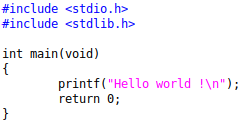
\includegraphics[scale=0.7, left]{\patchResults/hello_world_program}
	\end{center}
\end{figure}

\begin{figure}[H]
	\begin{center}
		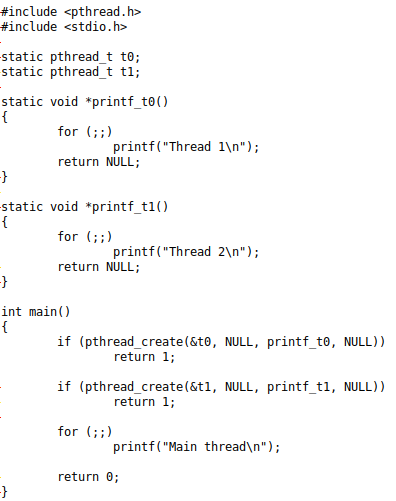
\includegraphics[scale=0.7, left]{\patchResults/thread_program}
	\end{center}
\end{figure}

%\newpage
%\section*{perf record -e cs\_etm/@tmc\_etf0/u --per-thread ./thread}
%Cet example montre le formatage dans la sortie standard suivant la commande
%\textbf{perf report --stdio}.

%\begin{figure}[H]
%        \begin{center}
%                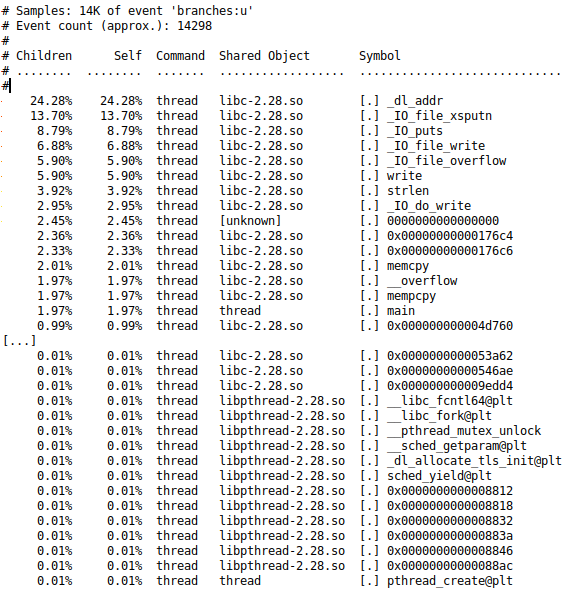
\includegraphics[width=\textwidth]{\patchResults/record_u_per_thread_thread}
%        \end{center}
%\end{figure}

%\newpage
%\section*{perf record -e cs\_etm/@tmc\_etf0/u --per-thread ./hello\_world}
%Cet example montre le formatage dans la sortie standard suivant la commande
%\textbf{perf report --stdio}.

%\begin{figure}[H]
%        \begin{center}
%                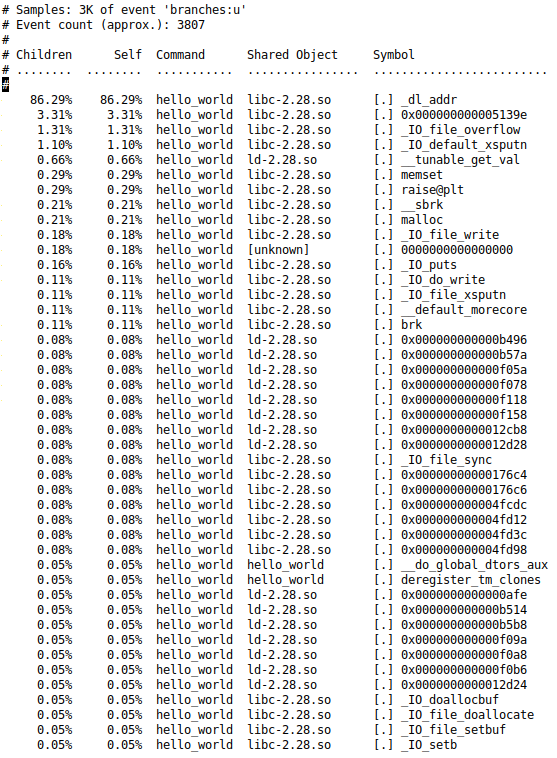
\includegraphics[width=\textwidth]{\patchResults/record_u_per_thread_hello_world}
%        \end{center}
%\end{figure}

%\newpage
%\section*{perf record -e cs\_etm/@tmc\_etf0,timestamp/k,branches --all-cpus ./hello\_world}
%Cet example montre le formatage dans la sortie standard suivant la commande
%\textbf{perf report --stdio}.

%\begin{figure}[H]
%        \begin{center}
%                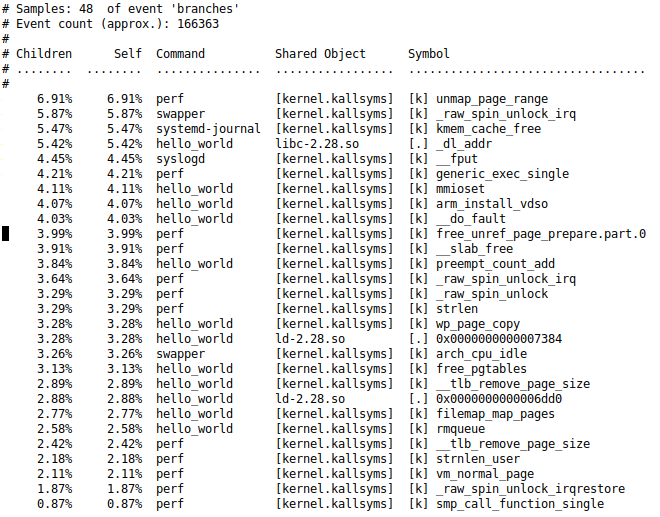
\includegraphics[width=\textwidth]{\patchResults/record_tmc_etf0_timestamp_k_branches_all_cpus_hello_world_0}
%        \end{center}
%\end{figure}

\newpage
\section*{perf record -vvv -e cs\_etm/contextid,freq,@tmc\_etf0/k,instructions --all-cpus ./hello\_world}
Cet example montre le formatage avec la librairie NCurses suivant la commande
\textbf{perf report}.

\begin{figure}[H]
	\begin{center}
		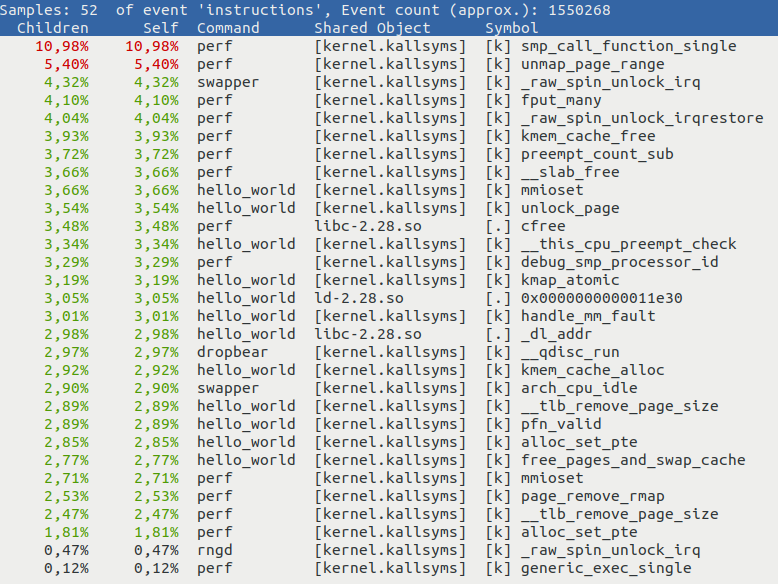
\includegraphics[width=\textwidth]{\patchResults/record_cs_etm_contextid_freq_@tmc_etf0_k_instructions_all_cpus_hello_world_0}
	\end{center}
\end{figure}

\begin{figure}[H]
	\begin{center}
		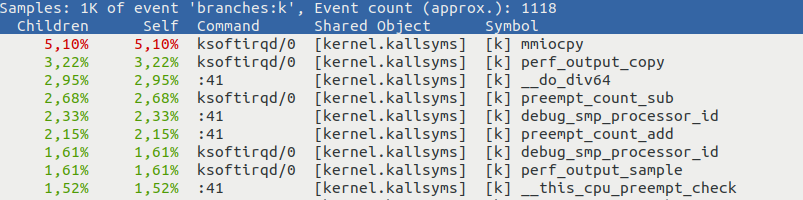
\includegraphics[width=\textwidth]{\patchResults/record_cs_etm_contextid_freq_@tmc_etf0_k_instructions_all_cpus_hello_world_1}
	\end{center}
\end{figure}

\begin{figure}[H]
	\begin{center}
		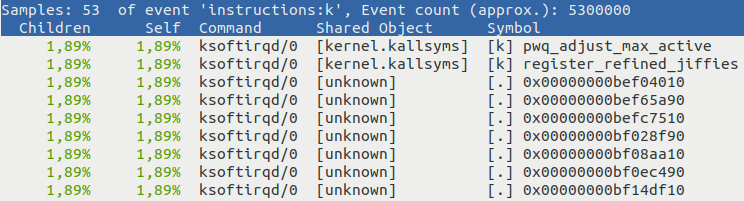
\includegraphics[width=\textwidth]{\patchResults/record_cs_etm_contextid_freq_@tmc_etf0_k_instructions_all_cpus_hello_world_2}
	\end{center}
\end{figure}





\appendix
%------
% Patch
%------

\chapter*{Patchs}
\addcontentsline{toc}{chapter}{Annexe 4 : Patchs}

Le patch est le moyen d'échanger et de communiquer les modifications faites
dans le code source du noyau Linux. Ce sont des fichiers générés par commande
GIT qui font état des différences entre les lignes retirées ou ajoutées.  La
granularité des modifications de GIT est par lignes. Ainsi si une ligne a été
modifiée, GIT le verra comme si une ligne avait été retirée puis ajoutée.  \\

\noindent
+ ceci est une ligne ajoutée \\
- ceci est une ligne retirée

Un exemple de patch est montré ci-dessous.\\

\section*{Patch 4 : coresight: etm3x: Enable timestamp if supported}
\begin{figure}[H]
	\begin{center}
		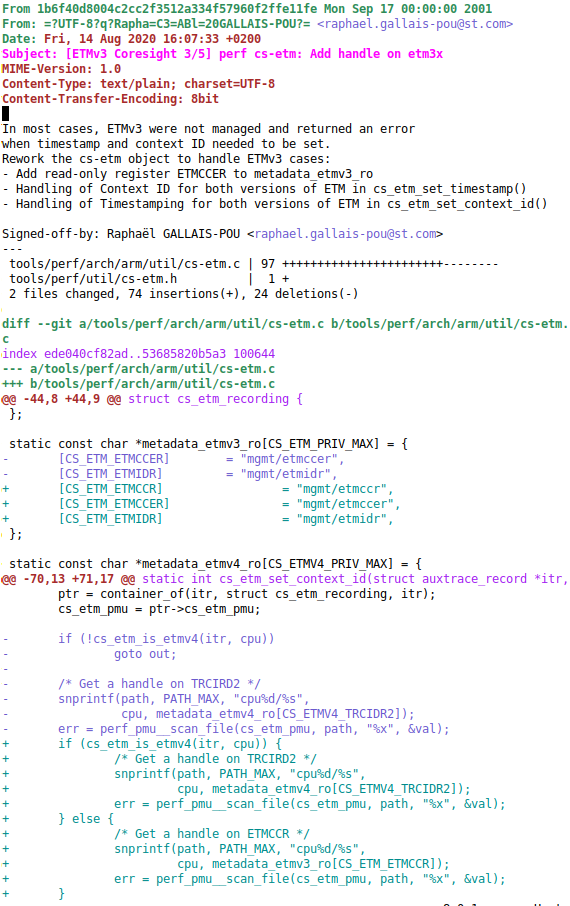
\includegraphics[width=\textwidth]{\pathPatchFour/0}
	\end{center}
\end{figure}

\begin{figure}[H]
	\begin{center}
		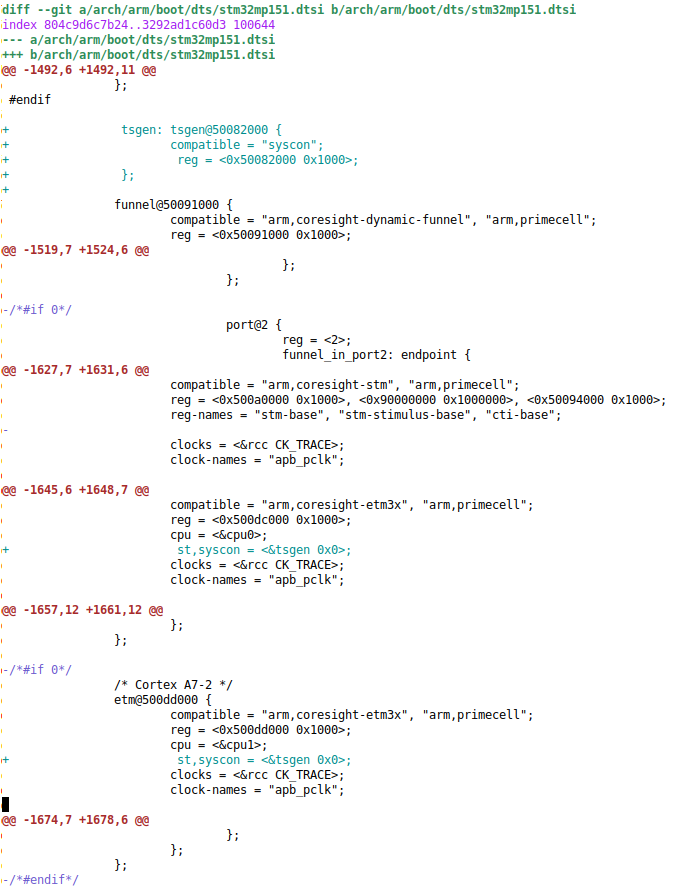
\includegraphics[width=\textwidth]{\pathPatchFour/1}
	\end{center}
\end{figure}

\begin{figure}[H]
	\begin{center}
		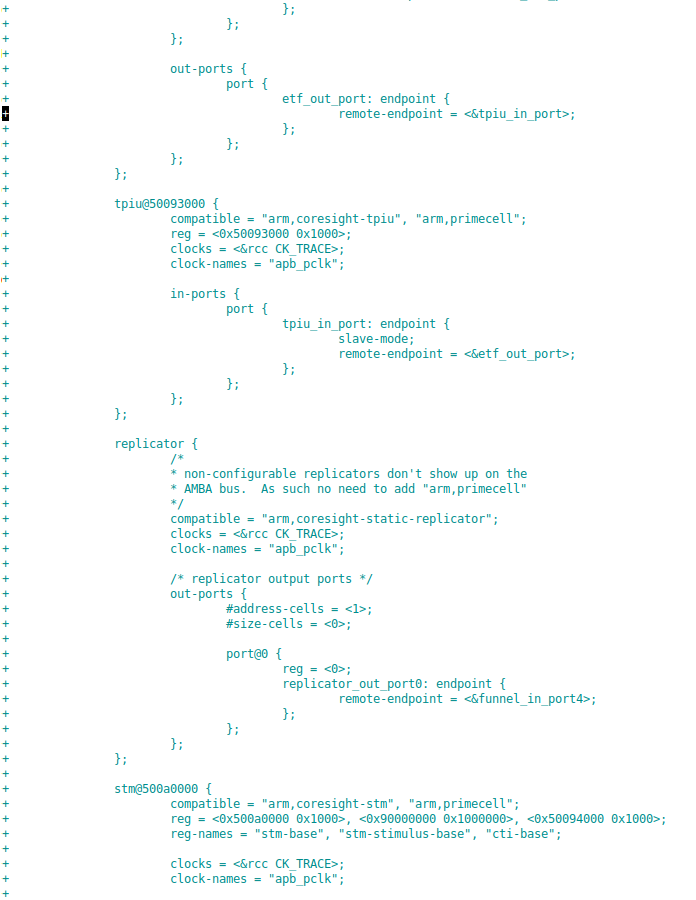
\includegraphics[width=\textwidth]{\pathPatchFour/2}
	\end{center}
\end{figure}

\begin{figure}[H]
	\begin{center}
		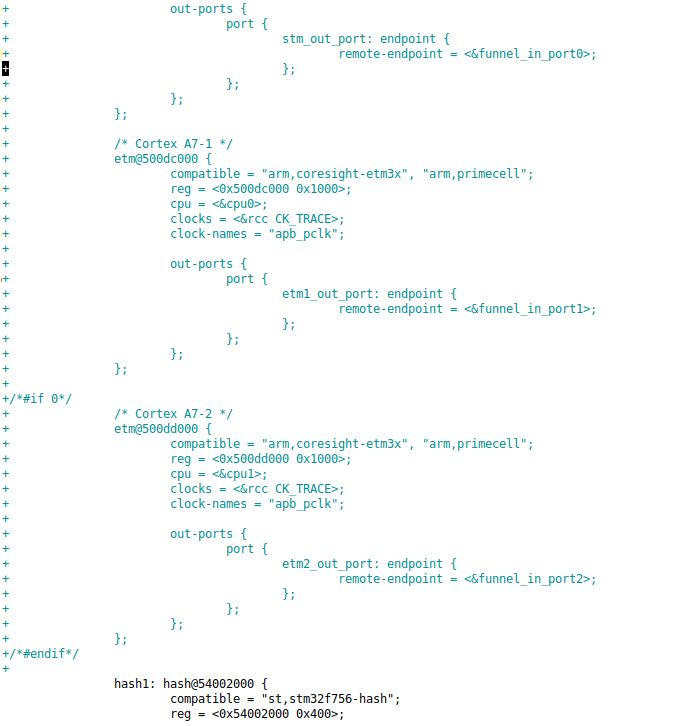
\includegraphics[width=\textwidth]{\pathPatchFour/3}
	\end{center}
\end{figure}


\appendix
\begin{figure}[H]
        \begin{center}
                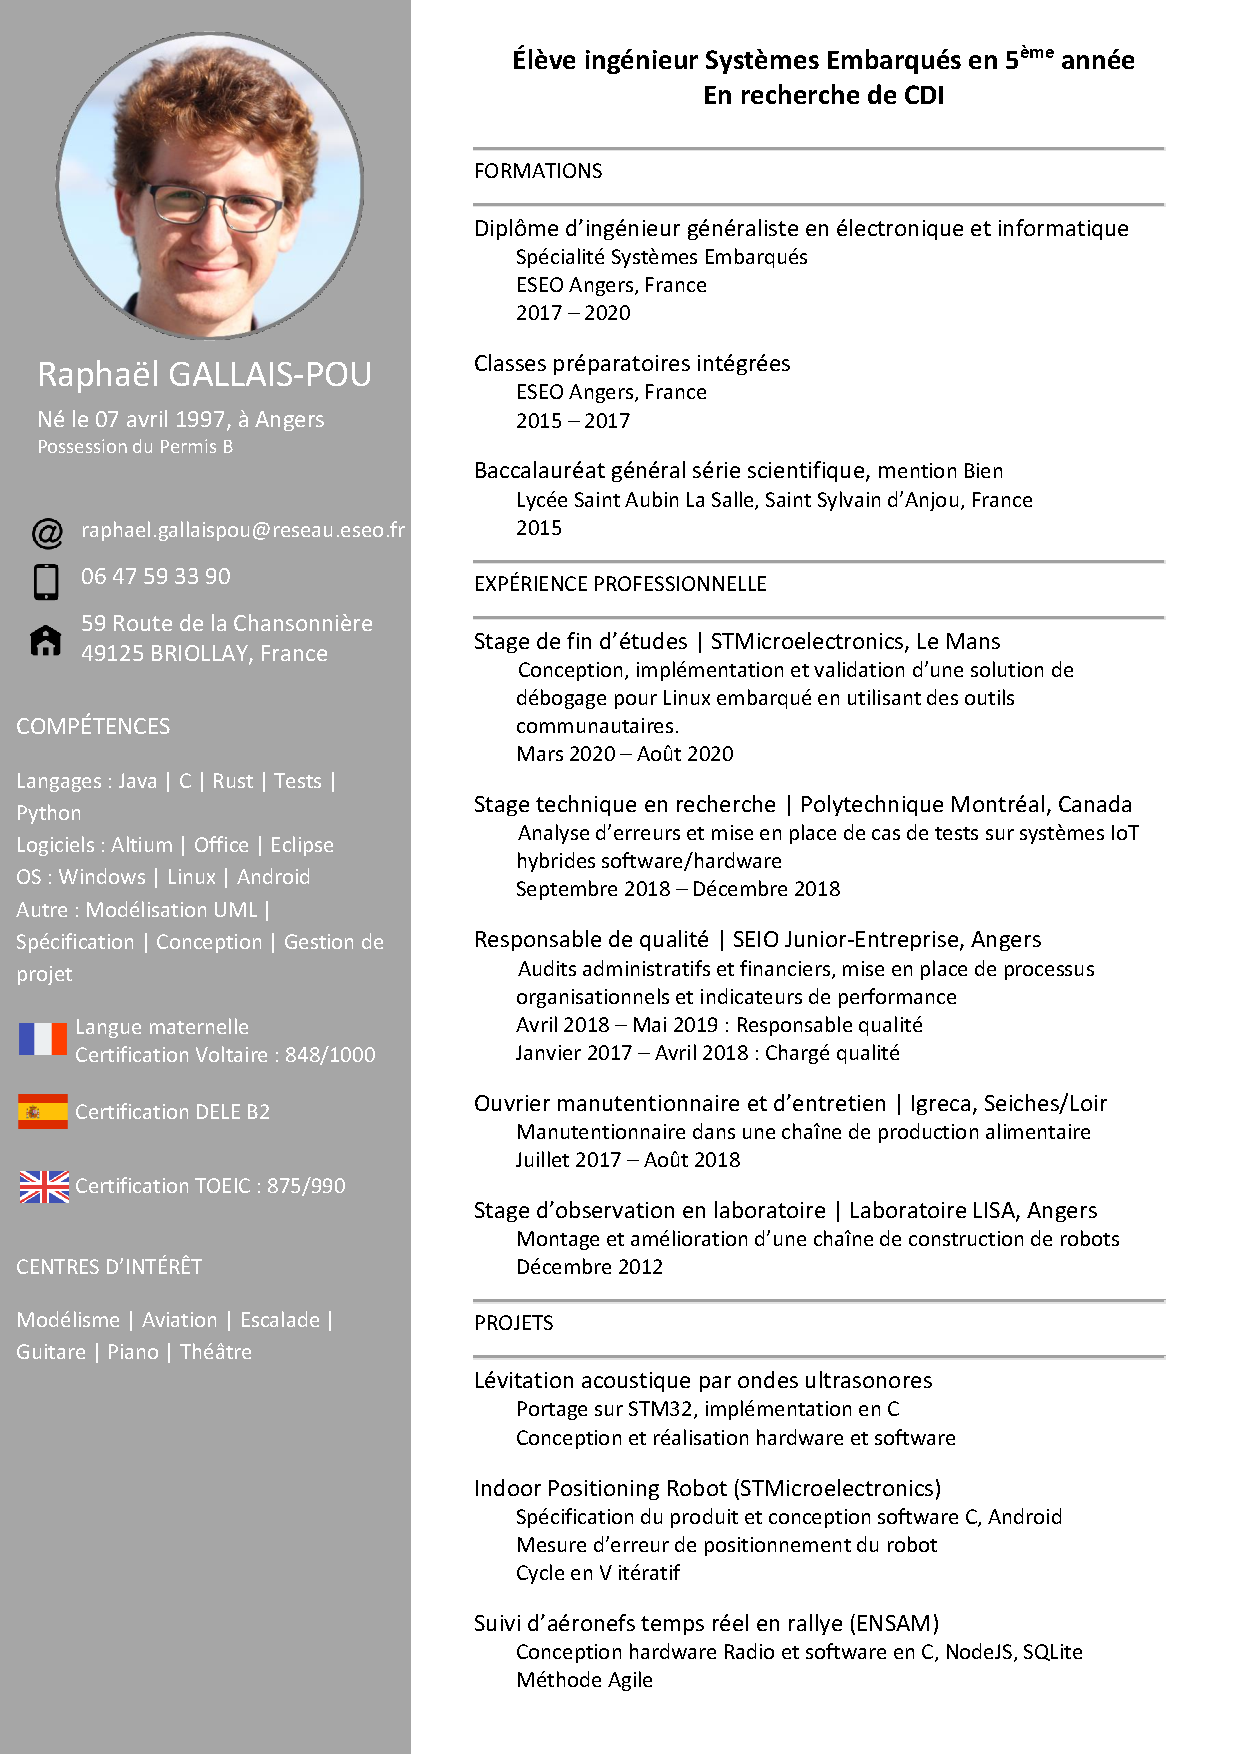
\includegraphics[width=\textwidth]{appendix/CV.pdf}
            \label{fig:Annexe : CV}
        \end{center}
\end{figure}
\addcontentsline{toc}{chapter}{Annexe 5 : CV}


\end{document}

% --- END ---

